\documentclass{article}  % use this instead for A4 paper
\usepackage{amsmath,amsfonts,amssymb}
\usepackage{authblk}
\usepackage{times}
\usepackage{float}
\restylefloat{table}  % https://stackoverflow.com/questions/1673942/latex-table-positioning
\usepackage{ifthen}
\usepackage{setspace}
\usepackage[super]{cite}[2003/11/04] % need vers. > 4.01
\usepackage{color}
\usepackage[colorlinks=true, allcolors=blue]{hyperref}
\usepackage{graphicx}
\graphicspath{ {./figures/} }
\usepackage{setspace}
\usepackage{tocloft}
\usepackage{doi}
\usepackage{csquotes}
\MakeOuterQuote{"}
\usepackage{pdflscape}
\usepackage{geometry}
\geometry{
  textwidth=11in,
  textheight=8.5in,
  headheight=0in,
  headsep=0in,
  marginparwidth=0in,
  papersize={11in,8.5in},
  left=0in,
  lmargin=0in,
  inner=0in,
  right=0in,
  rmargin=0in,
  outer=0in,
  top=0in,
  tmargin=0in,
  bottom=0in,
  bmargin=0in,
}

\newcommand{\code}[1]{\small \texttt{#1} \normalsize}
\newcommand{\tcode}[1]{\footnotesize \texttt{#1} \normalsize}

\pagestyle{empty}               % page numbers is default; use empty for no numbers


\title{Supplementary Material}

\author[a]{Derek Berger}
\author[a,*]{Jacob Levman}
\author[b]{Gurpreet M. Matharoo}
\affil[a]{St. Francis Xavier University, Department of Computer Science, 4130 University Avenue, Antigonish, Canada, B2G 2W5}
\affil[b]{St. Francis Xavier University, ACENET, 4130 University Avenue, Antigonish, Canada, B2G 2W5}


\renewcommand{\cftdotsep}{\cftnodots}
\cftpagenumbersoff{figure}
\cftpagenumbersoff{table}

\begin{document}

\begin{center}
\maketitle
\end{center}



% \begin{spacing}{1}   % use single spacing for supplementary


\begin{figure}[H]
\begin{center}
\includegraphics[width=\textwidth,height=0.9\textheight,keepaspectratio]{all_by_fine_feature_groups.png}
\end{center}
\caption
{ \label{fig:feature-group-all}
AUROC distributions across gross feature groupings and comparison tasks.}
\end{figure}





\begin{figure}[H]
\begin{center}
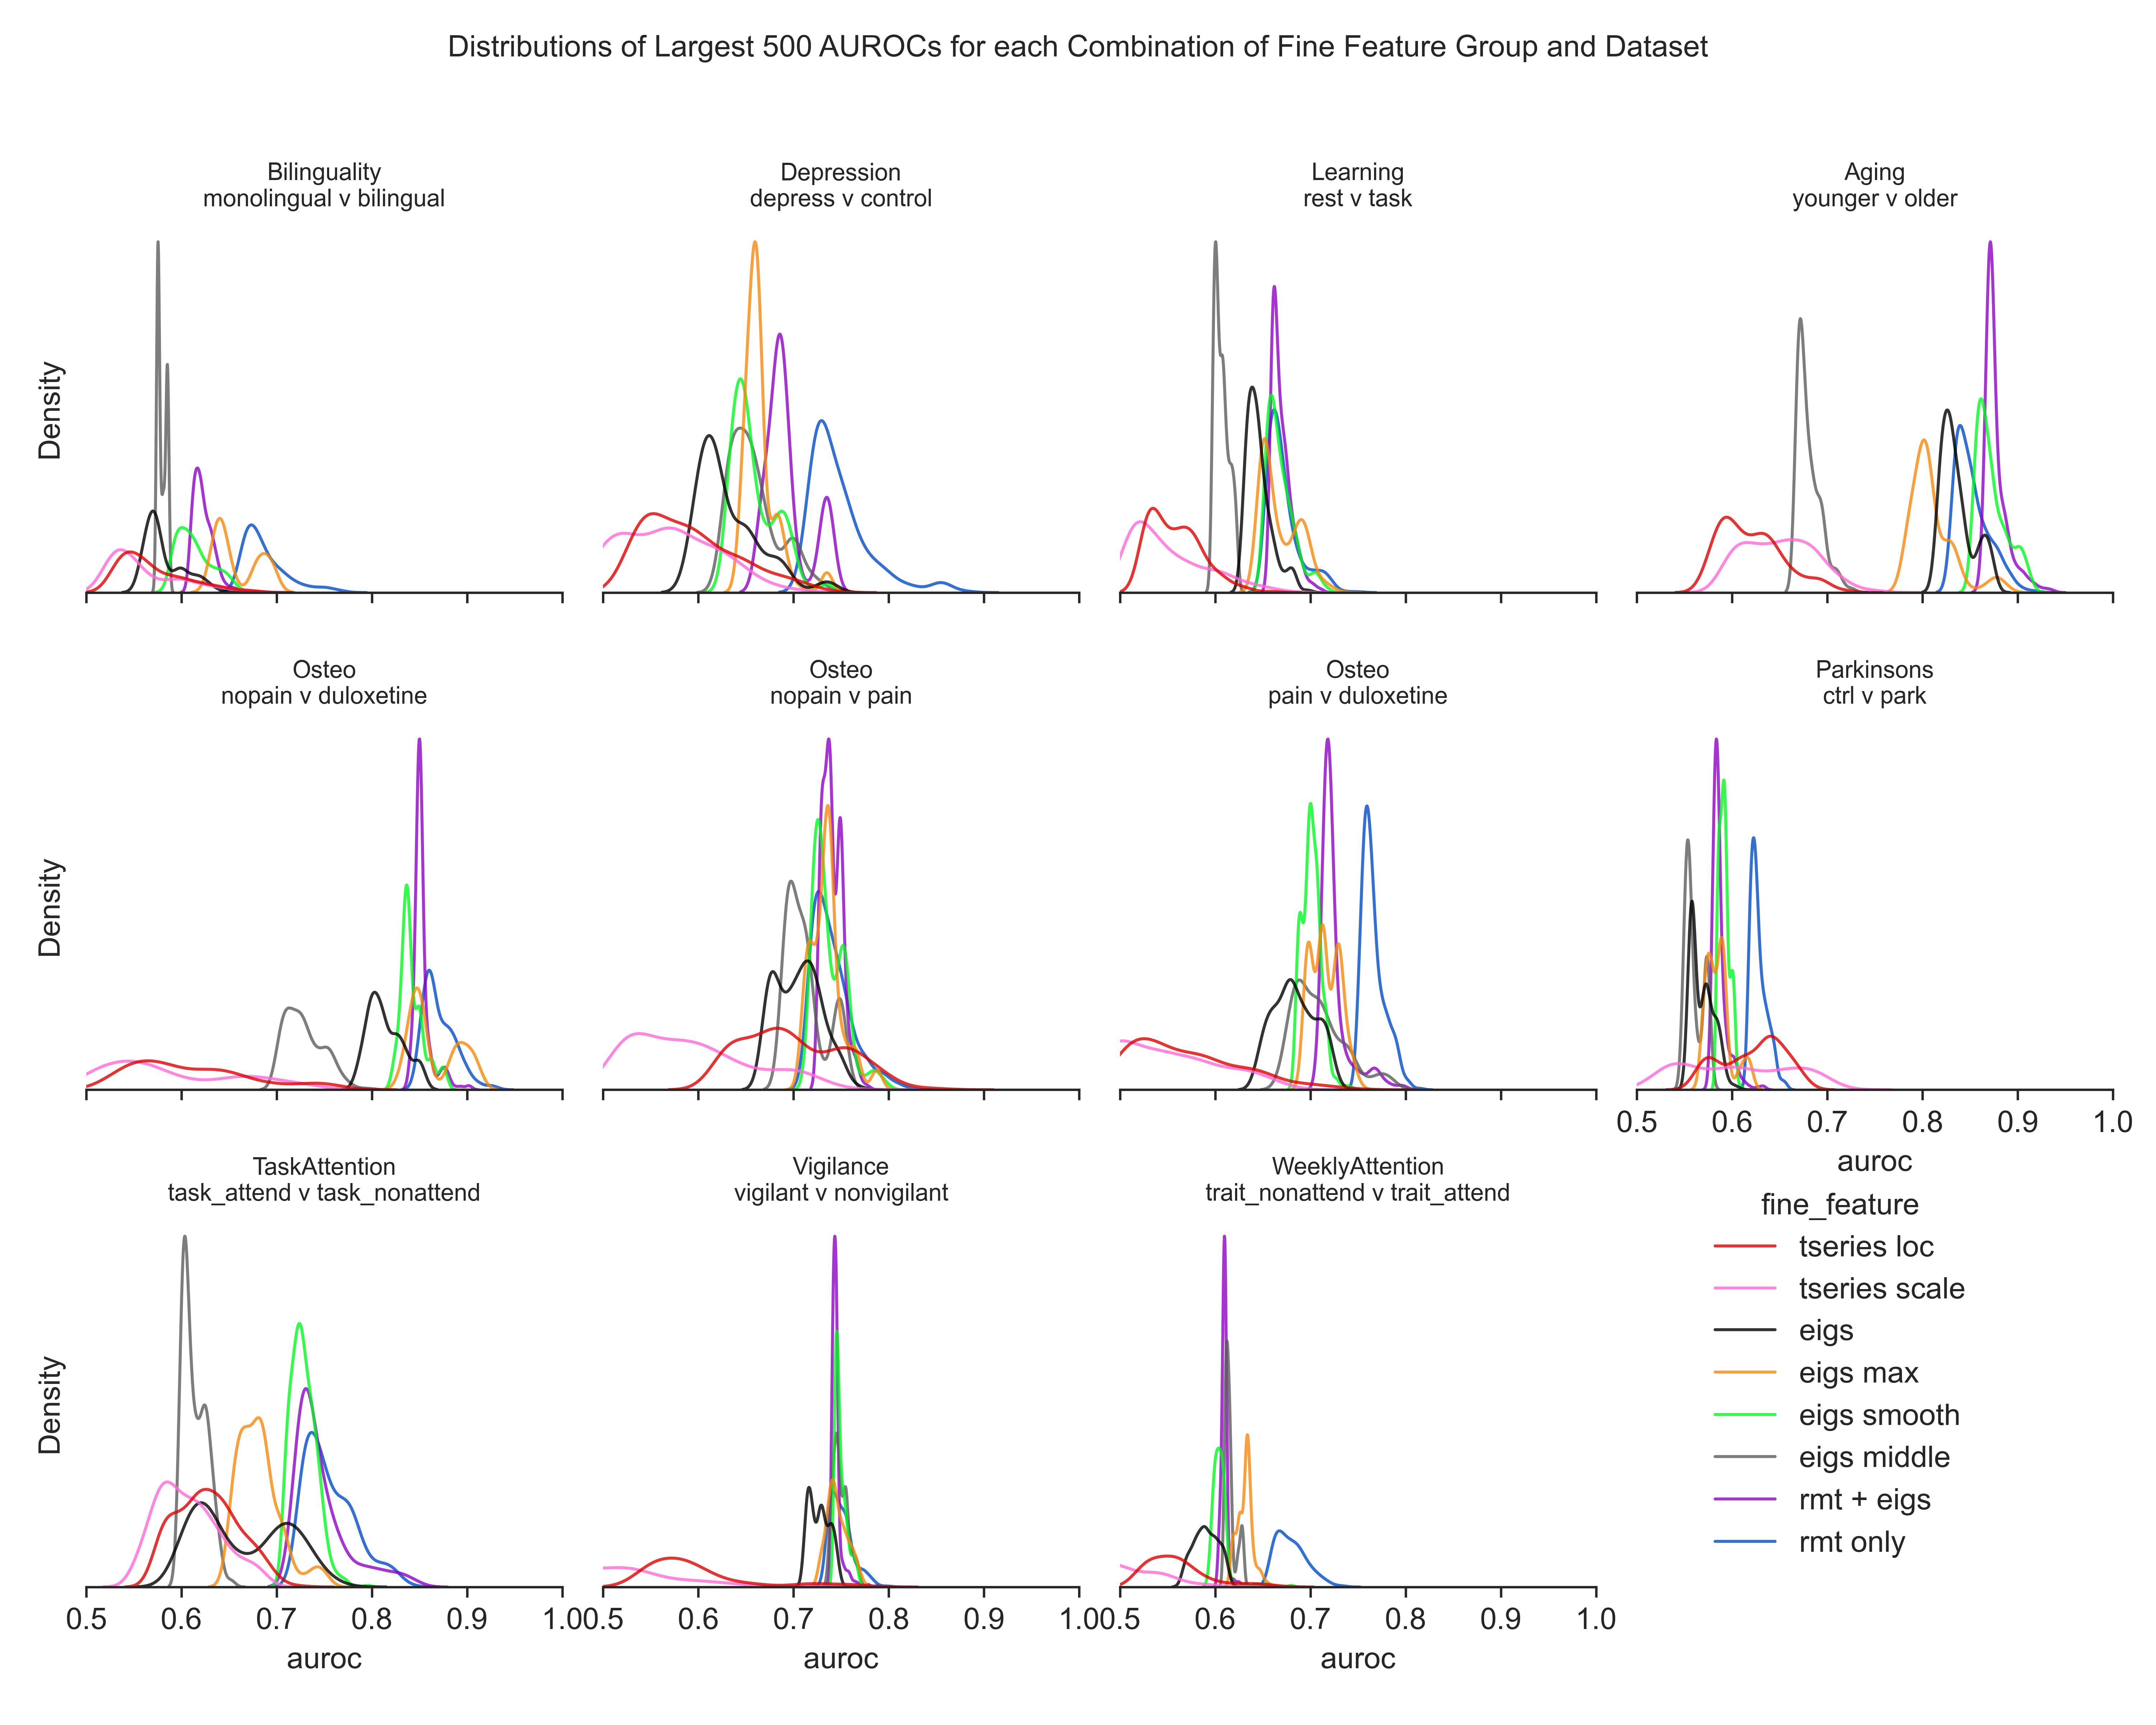
\includegraphics[width=\textwidth,height=0.9\textheight,keepaspectratio]{fine_feature_largest_by_subgroup.png}
\end{center}
\caption
{ \label{fig:fine-largest} Distributions of largest 500 mAUROCs across fine
feature grouping, by comparison task. Note "rmt only" and "rmt + eigs" features
tend to have the best possible performances across predictable tasks. }
\end{figure}



\begin{figure}[H]
\begin{center}
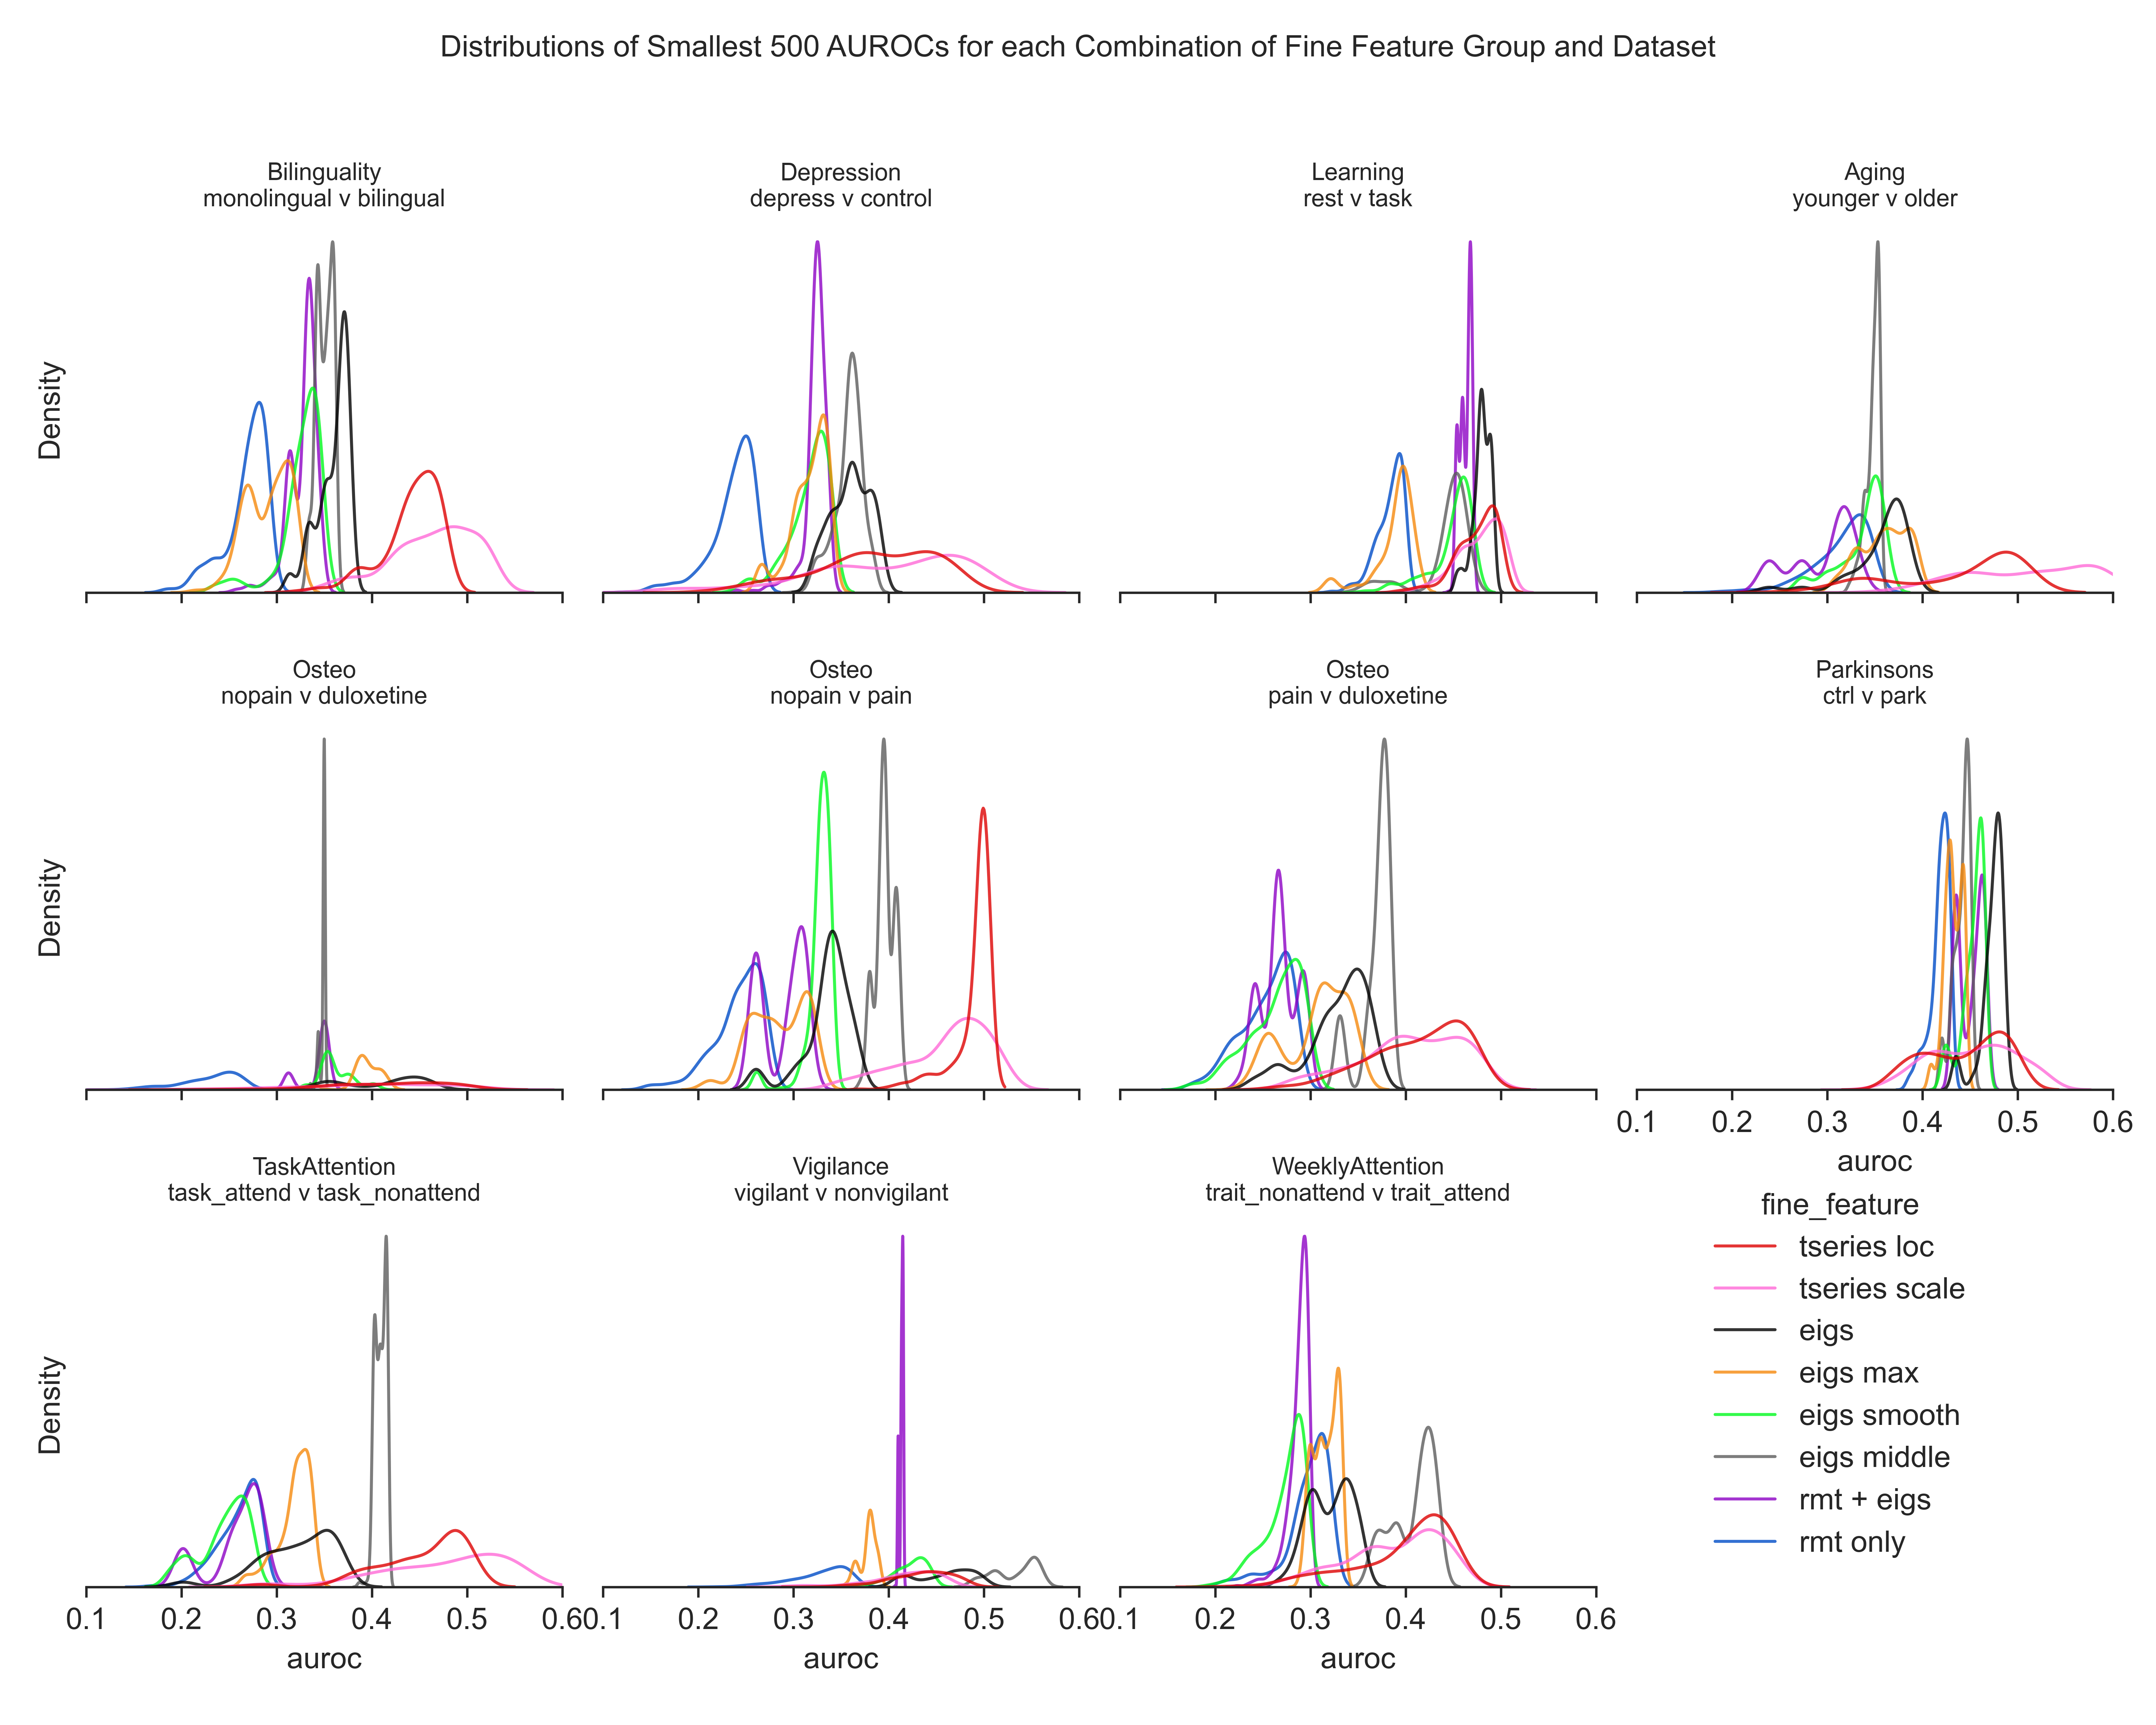
\includegraphics[width=\textwidth,height=0.9\textheight,keepaspectratio]{fine_feature_smallest_by_subgroup.png}
\end{center}
\caption
{ \label{fig:fine-smallest} Distributions of smallest 500 mAUROCs across fine
feature groupings, by comparison task. Note "rmt only" and "rmt + eigs"
features tend to have the worse possible performances across predictable
tasks.}
\end{figure}



\begin{figure}[H]
\begin{center}
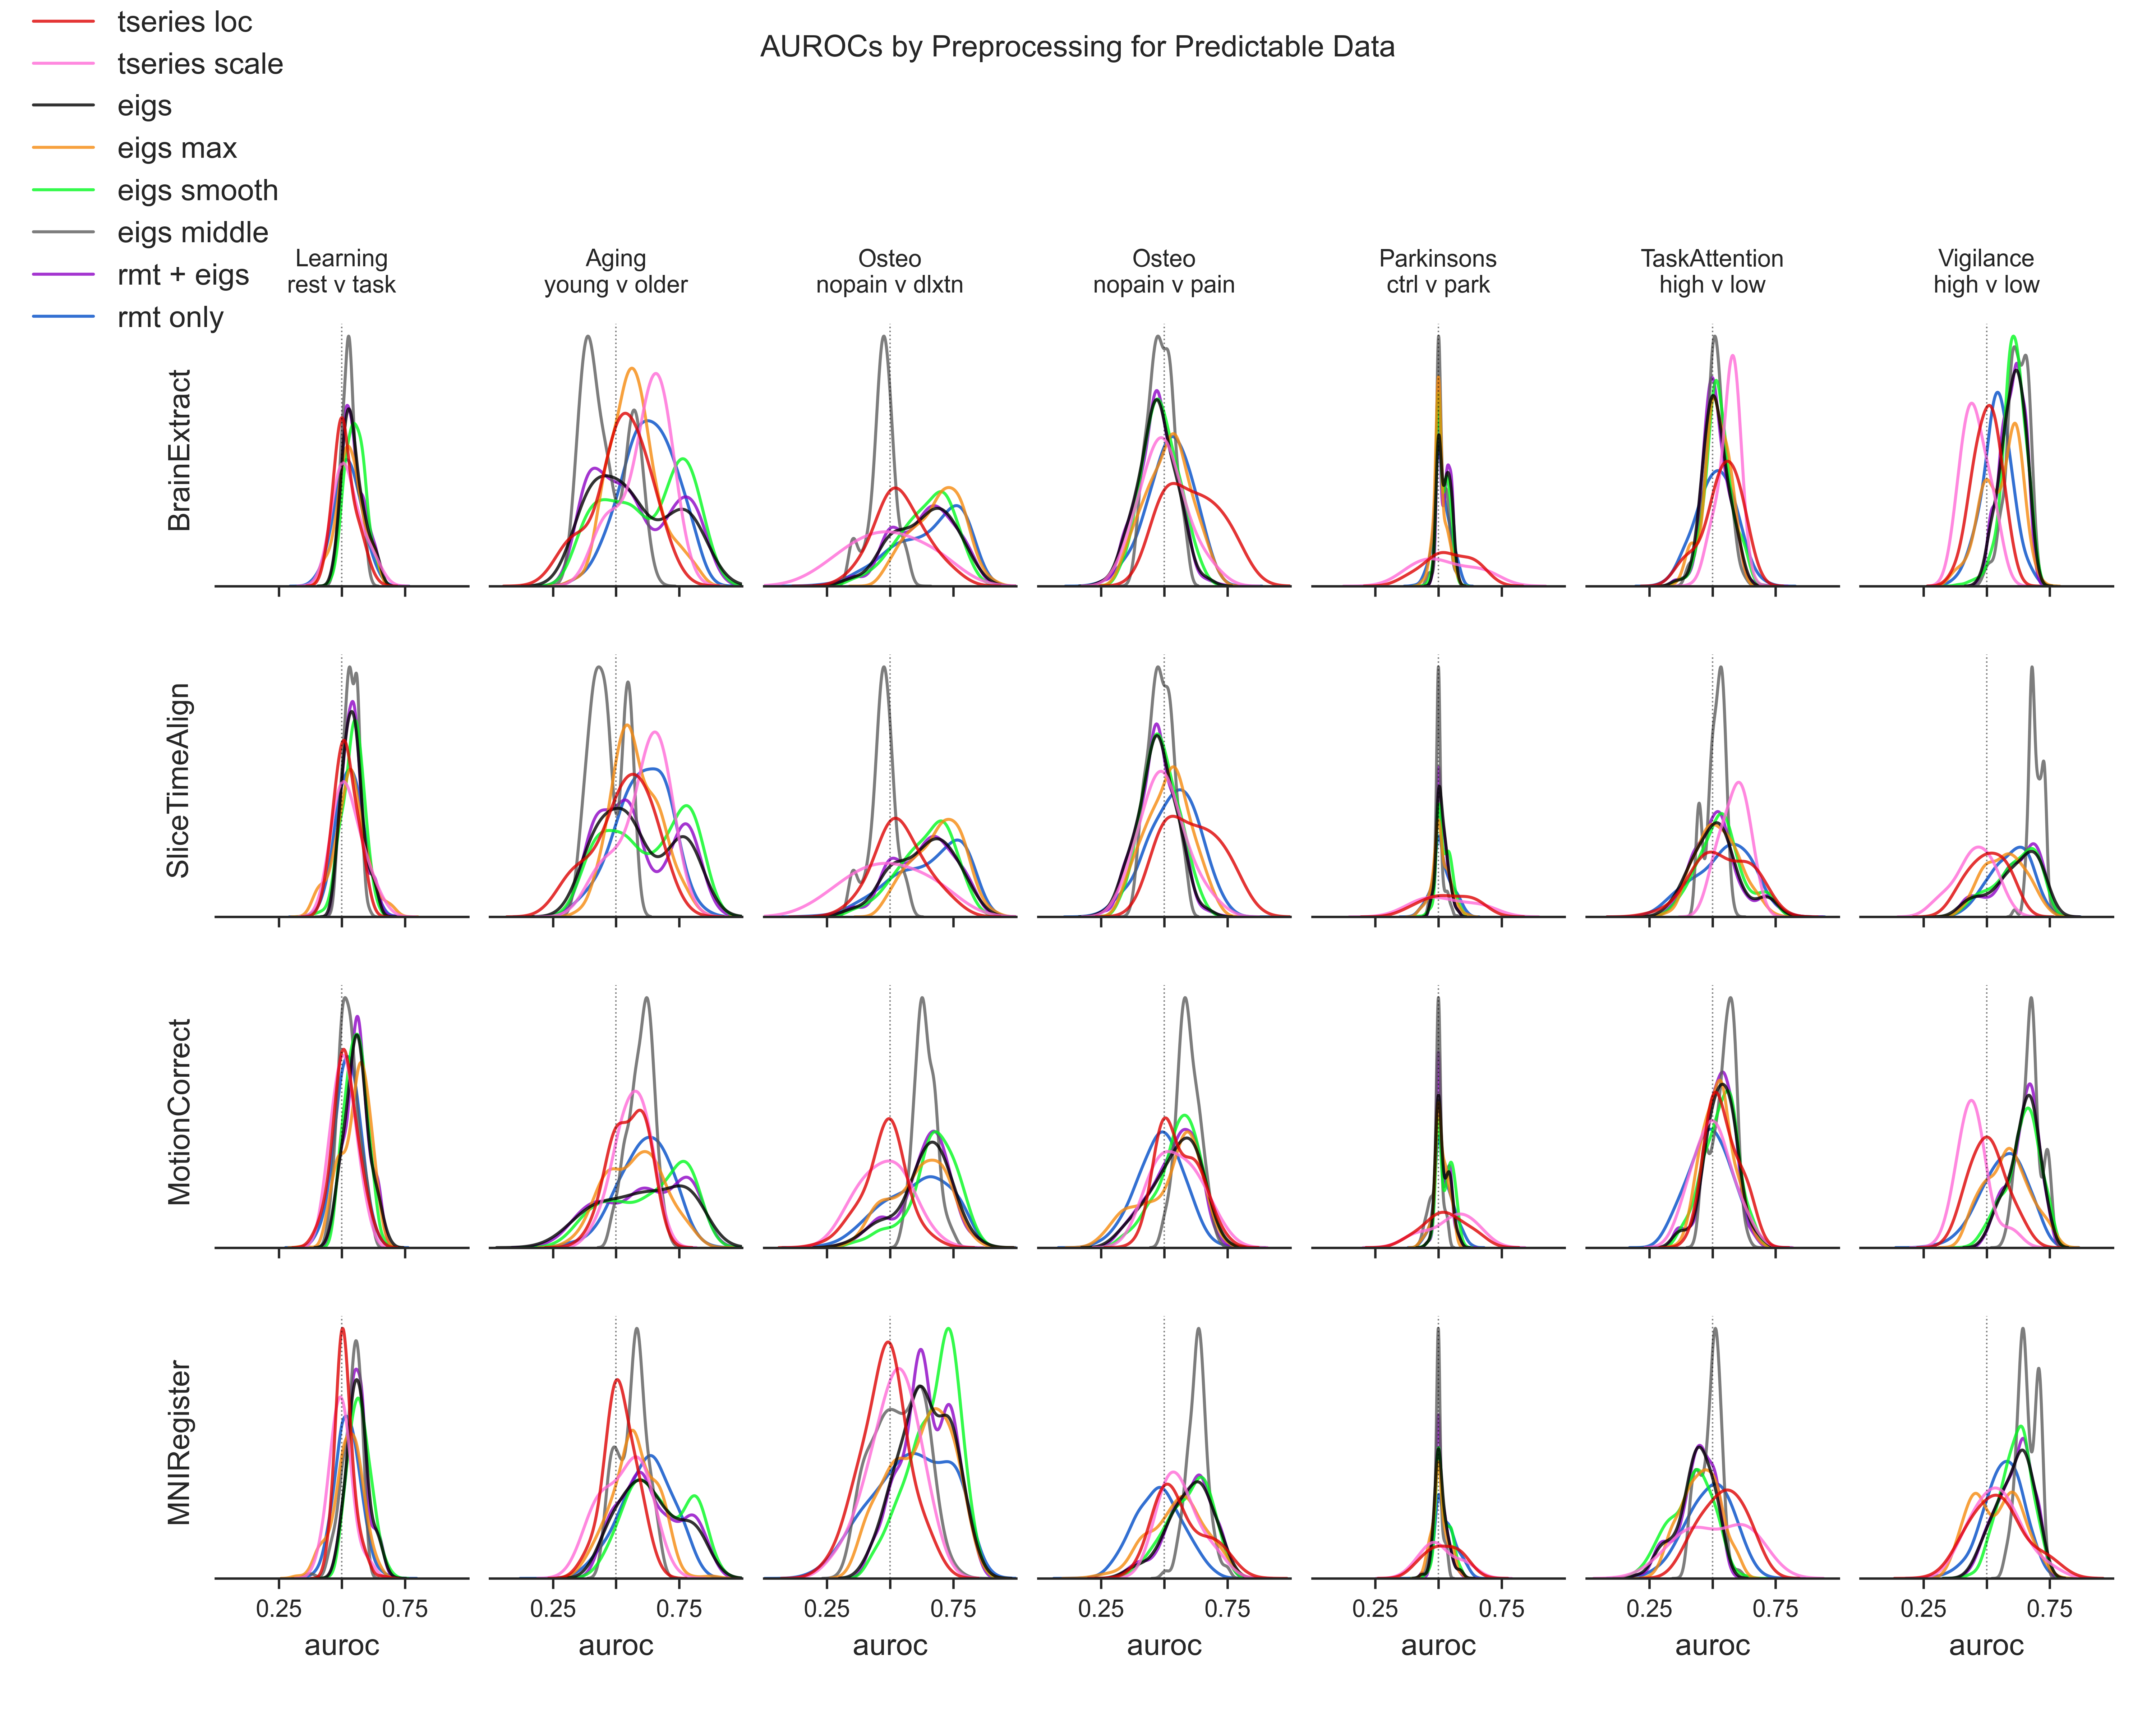
\includegraphics[width=\textwidth,height=0.9\textheight,keepaspectratio]{fine_feature_by_preproc_predictive_subgroup.png}
\end{center}
\caption
{ \label{fig:fine-preproc}
AUROC distributions across fine feature groupings and predictable comparison tasks, with effect of preprocessing.}
\end{figure}


\begin{figure}[H]
\begin{center}
\includegraphics[width=\textwidth,height=0.9\textheight,keepaspectratio]{coarse_feature_group_by_predictive_subgroup_classifier.png}
\end{center}
\caption
{ \label{fig:coarse-classifier} AUROC distributions across coarse feature
groupings and predictable comparison tasks, by classifier. Note the general
similarity of each distribution within a particular classification task
(column) and within each feature grouping.}
\end{figure}



\begin{figure}[H]
\begin{center}
\includegraphics[width=\textwidth,height=0.9\textheight,keepaspectratio]{fine_feature_group_by_predictive_subgroup_classifier.png}
\end{center}
\caption
{ \label{fig:fine-classifier} AUROC distributions across fine feature groupings
and predictable comparison tasks, by classifier. Note the general similarity of
each distribution within a particular classification task (column) and within
each feature grouping. Note also that, within a classification task (column),
that the rank ordering of features, based on wither the median, mode, or mean,
does not change dramatically or consistently from classifier to classifier. }
\end{figure}

\begin{figure}[H]
\begin{center}
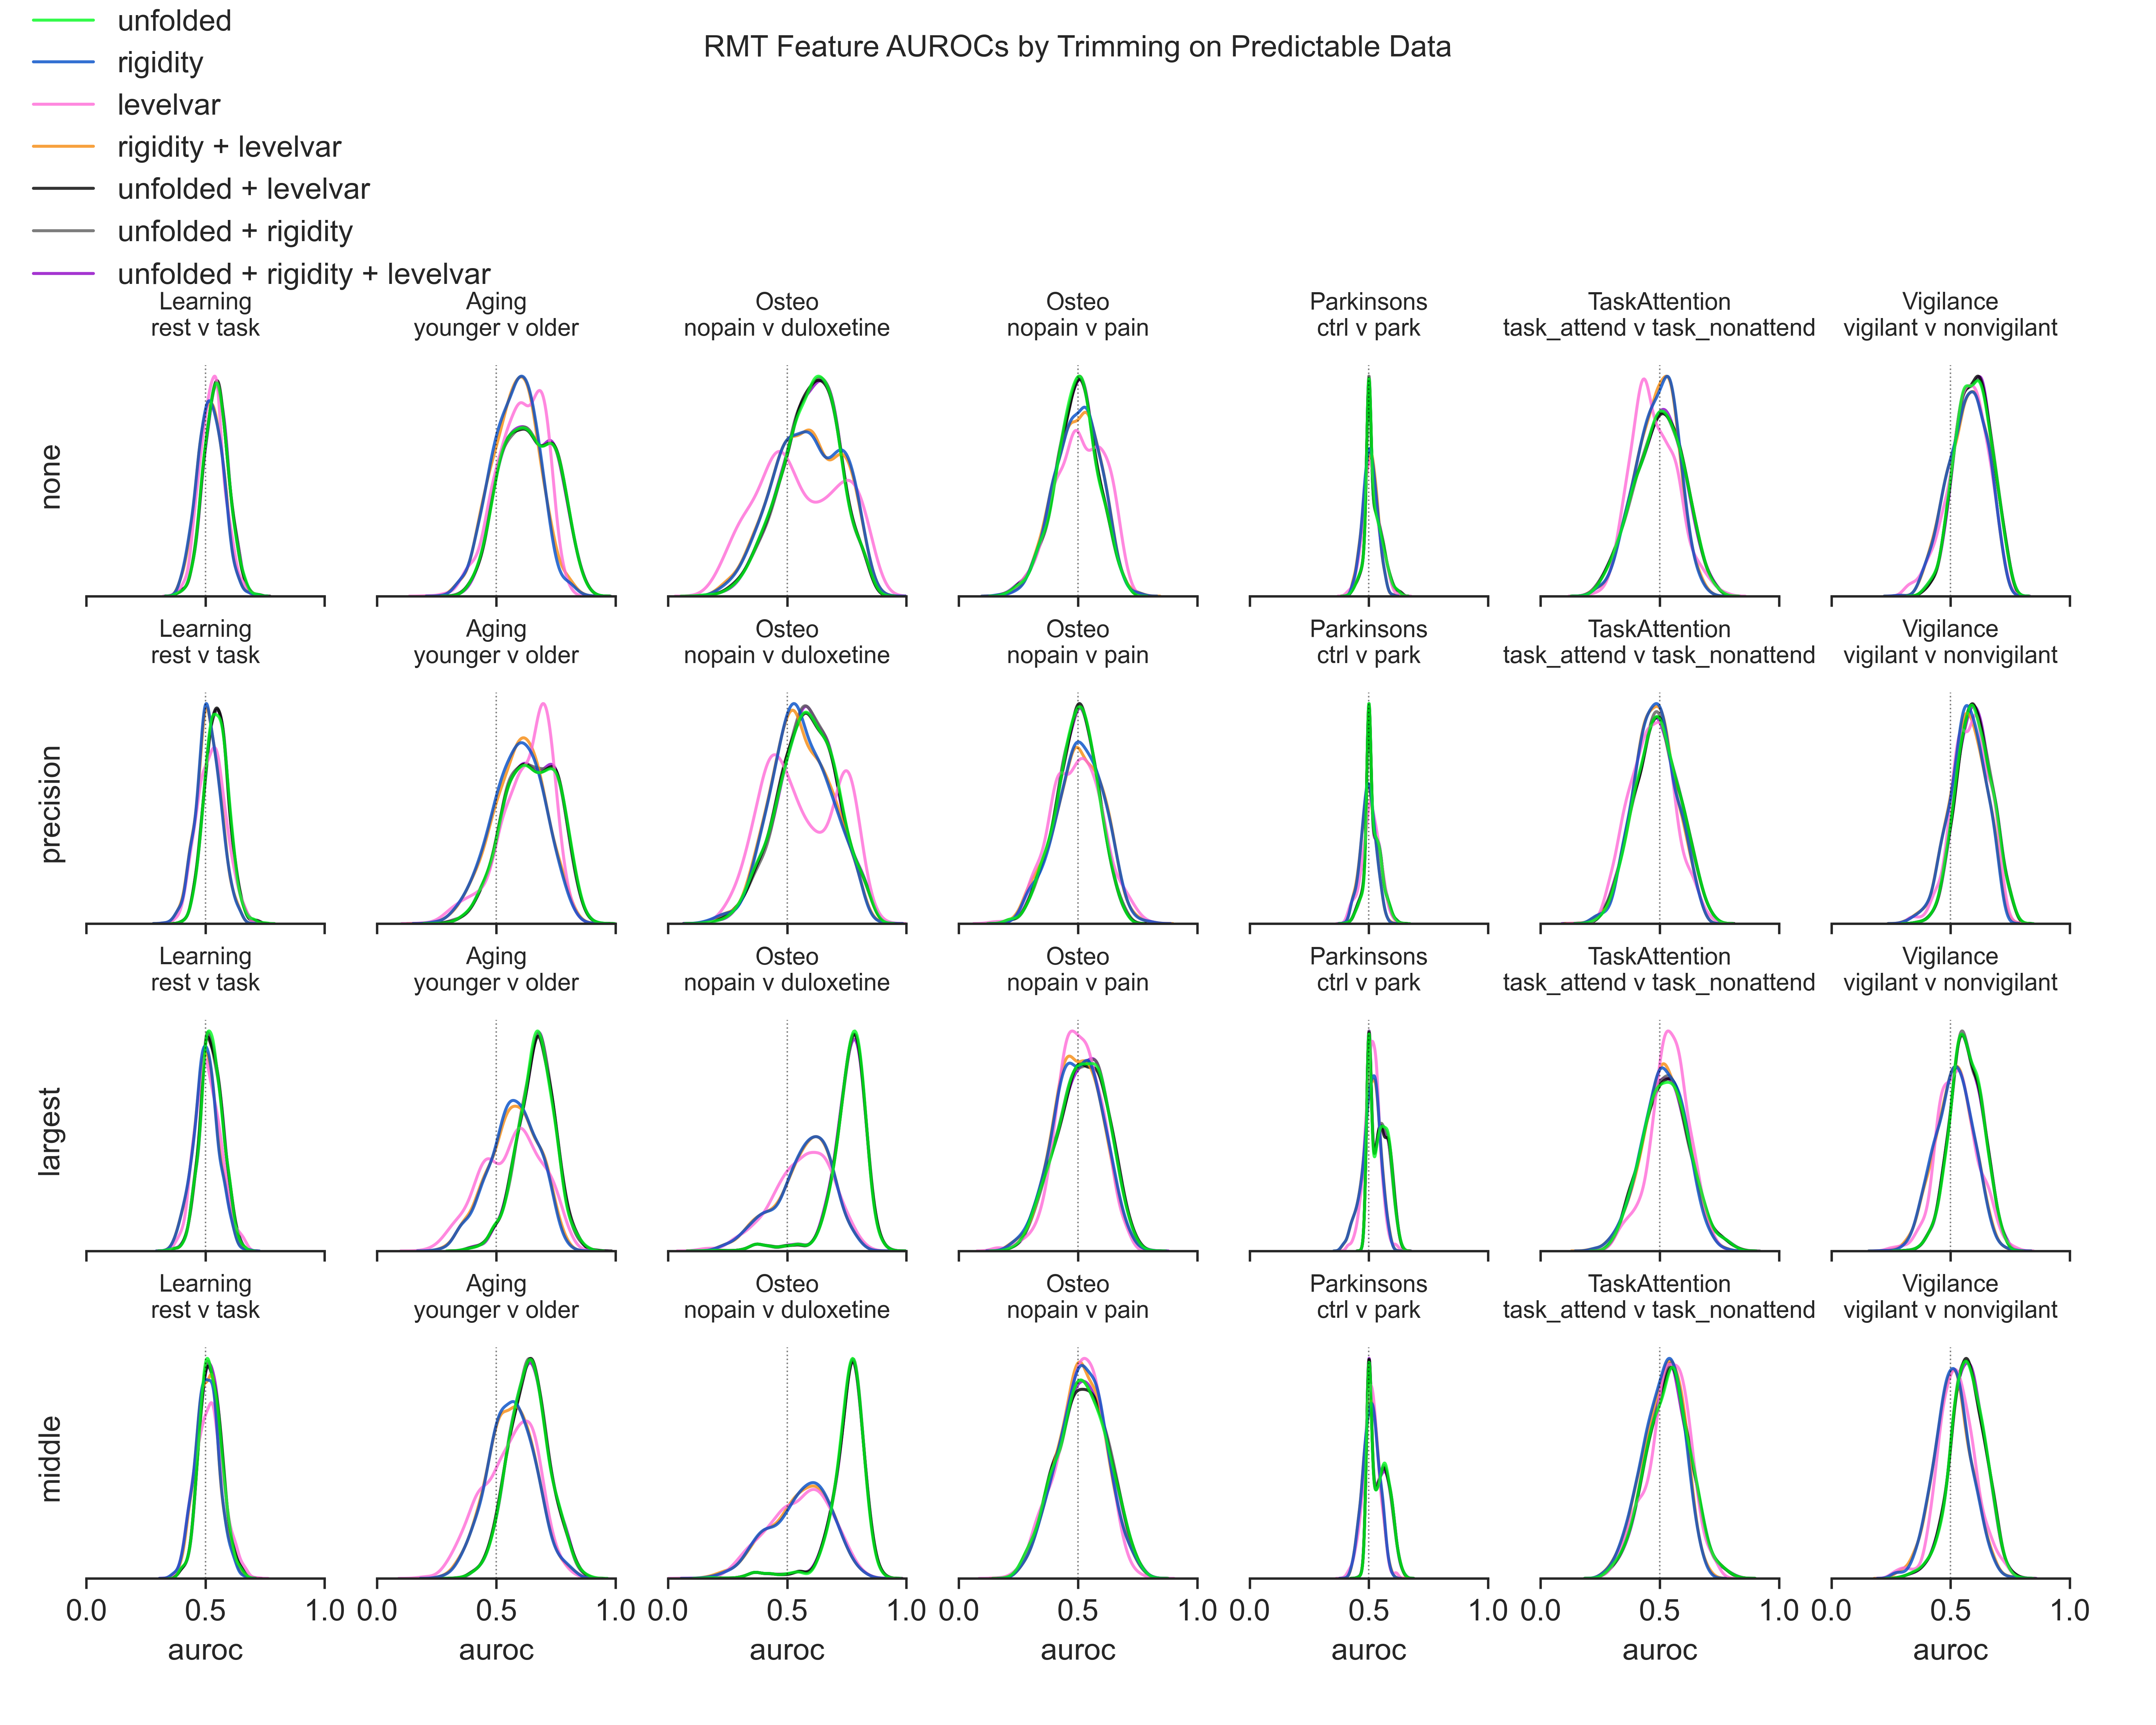
\includegraphics[width=\textwidth,height=0.9\textheight,keepaspectratio]{rmt_feature_auroc_by_trim.png}
\end{center}
\caption
{ \label{fig:fine-trim} Distributions of mAUROCs for unfolding-dependent RMT
features, by trimming. Note the tendency for a rightward shift in the mAUROC
distributions of the features involving the unfolded eigenvalues when using
largest or middle trimming (most dramatic in the Osteo nopain v duloxetine
condition). The impact of these trimming methods on the rigidity and level
variance features, however, was mixed (compare Vigilance data to Osteo nopain v
duloxetine condition.)}
\end{figure}



\begin{figure}[H]
\begin{center}
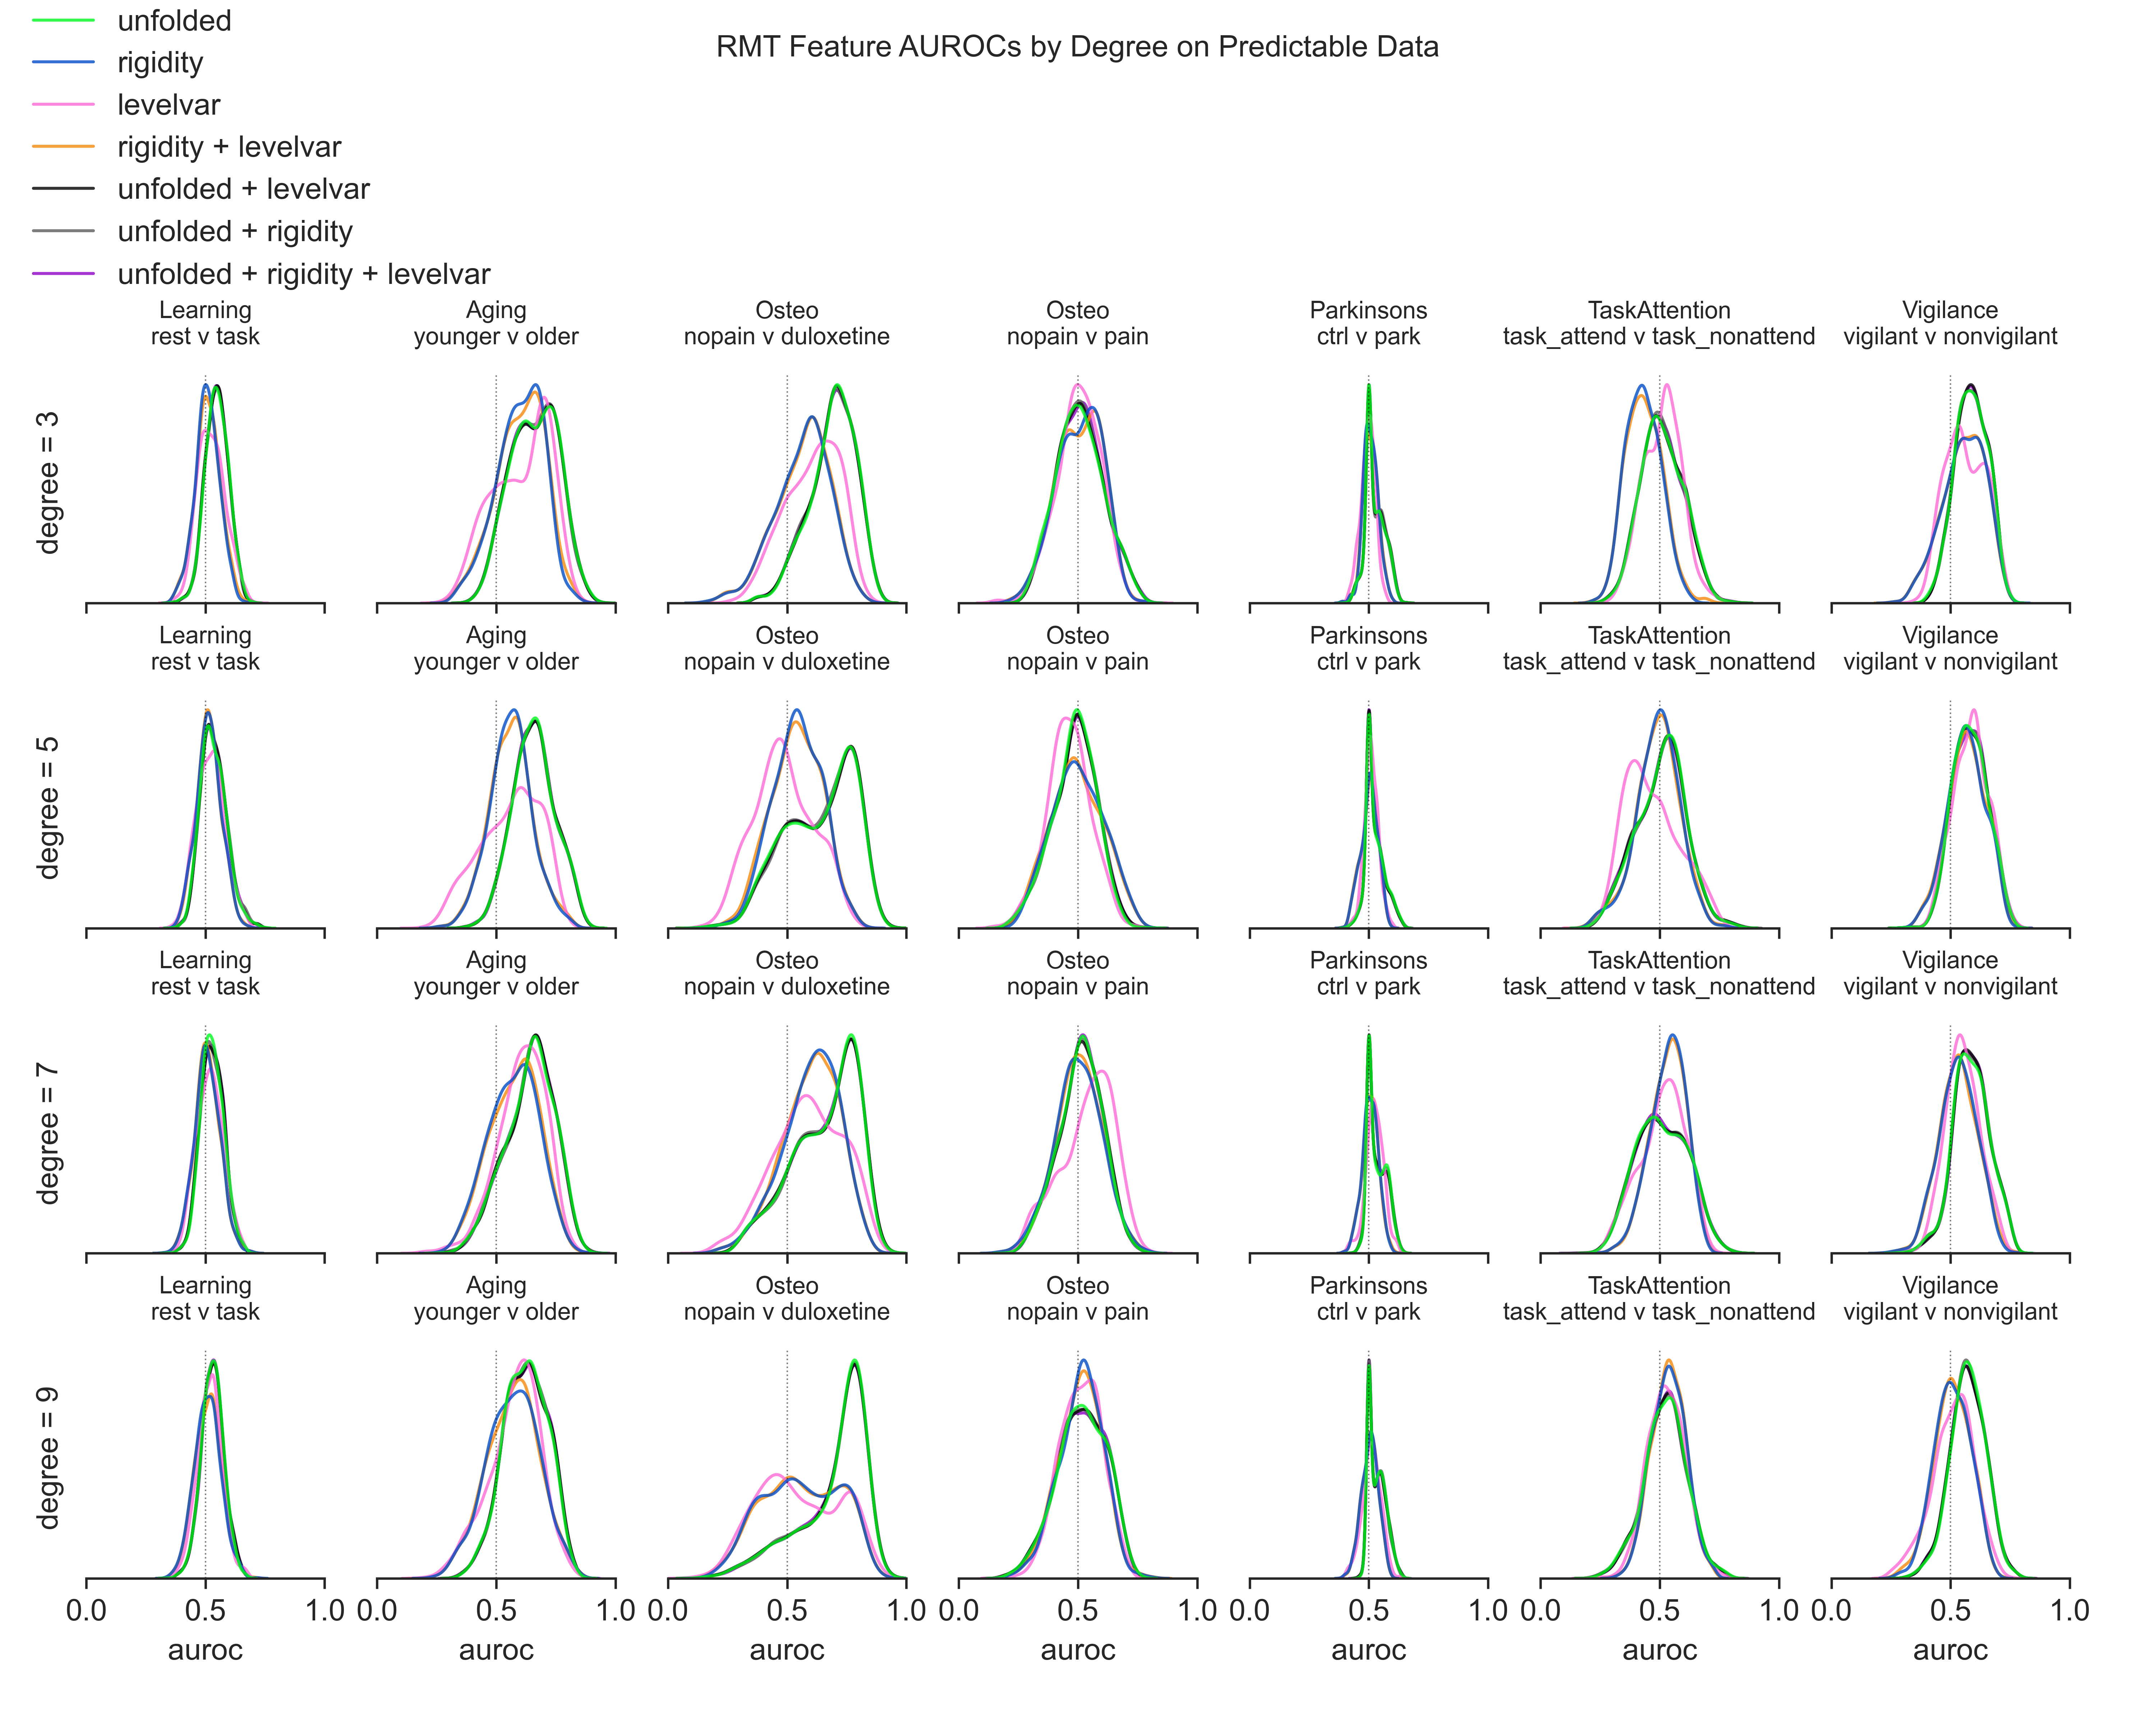
\includegraphics[width=\textwidth,height=0.9\textheight,keepaspectratio]{rmt_feature_auroc_by_degree.png}
\end{center}
\caption
{ \label{fig:fine-degree}
Distributions of mAUROCs for unfolding-dependent RMT features, by degree.}
\end{figure}


\begin{figure}[H]
\begin{center}
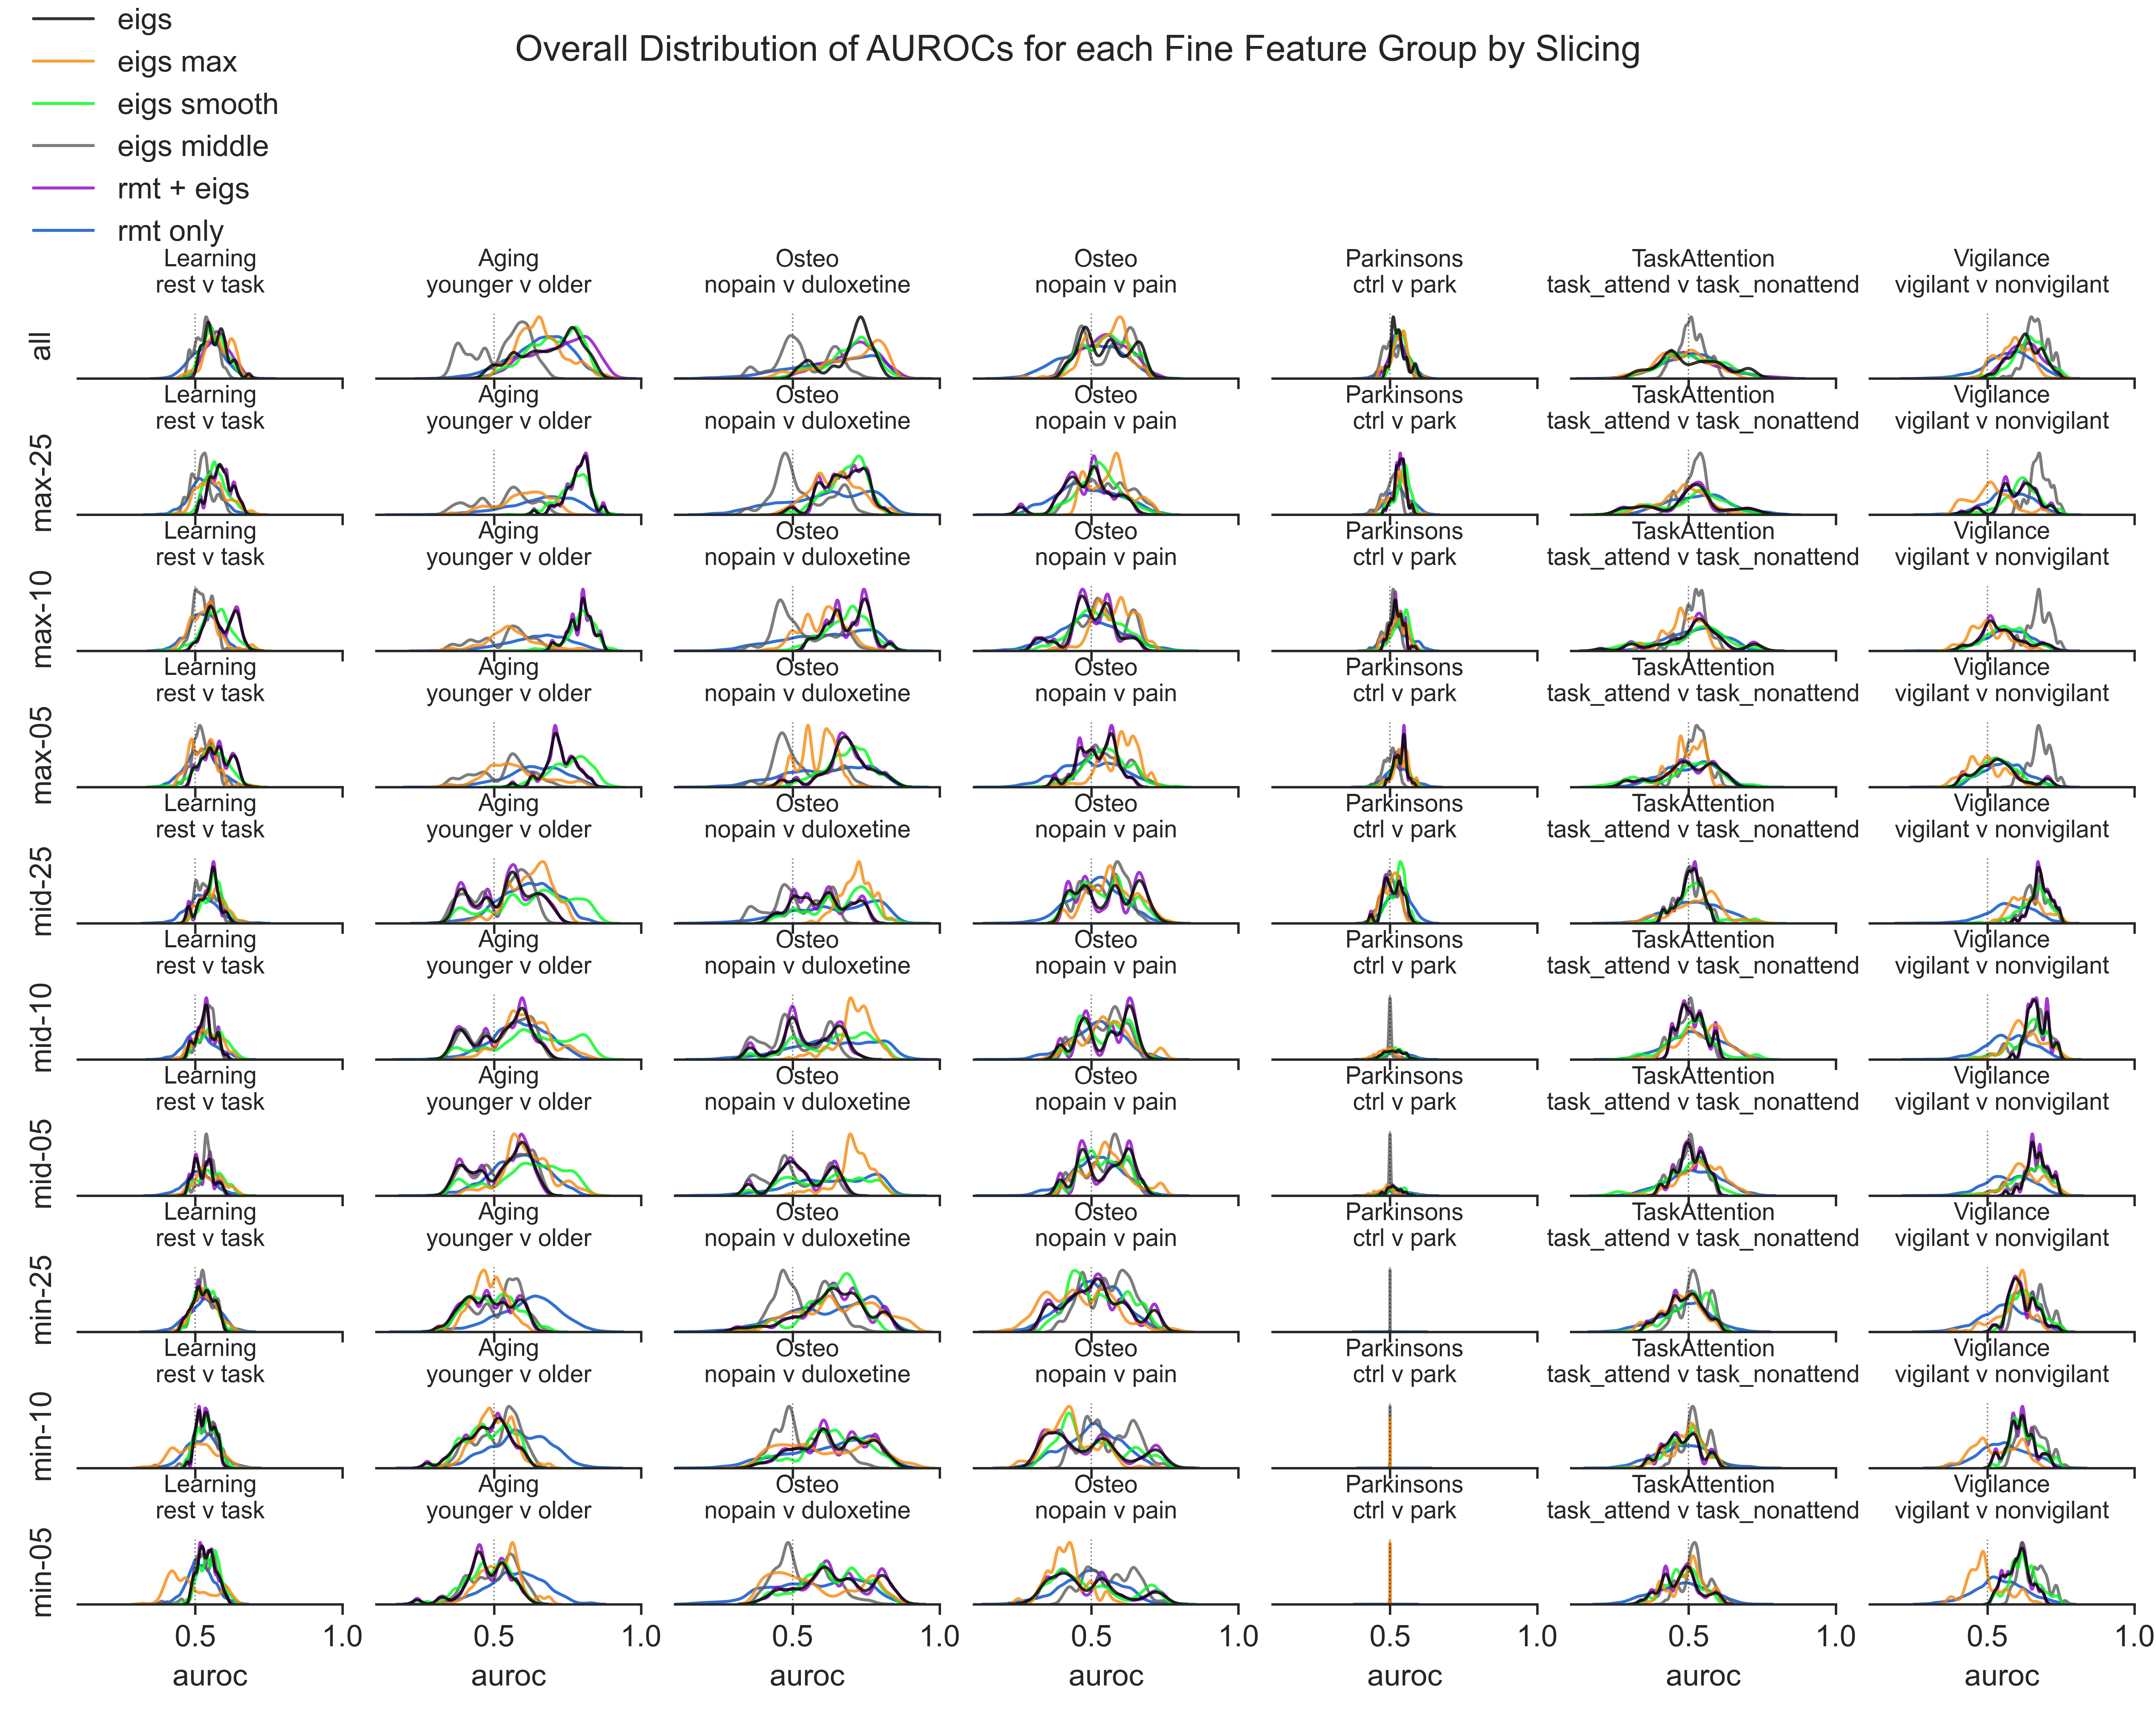
\includegraphics[width=\textwidth,height=0.9\textheight,keepaspectratio]{rmt_eigs_aurocs_by_subgroup_and_slicing.png}
\end{center}
\caption
{ \label{fig:best-params-slicing} Distributions of mAUROCs by slicing. Features
involving the full spectrum (raw eigenvalues, smoothed eigenvalues, and rmt +
eigs) sometimes have most positive mAUROC distributions when using the larger
eigenfeature values (first three columns) or middle values (Osteo nopain v pain
condition, Vigilance classification task).}
\end{figure}

% \begin{figure}[H]
% \begin{center}
% 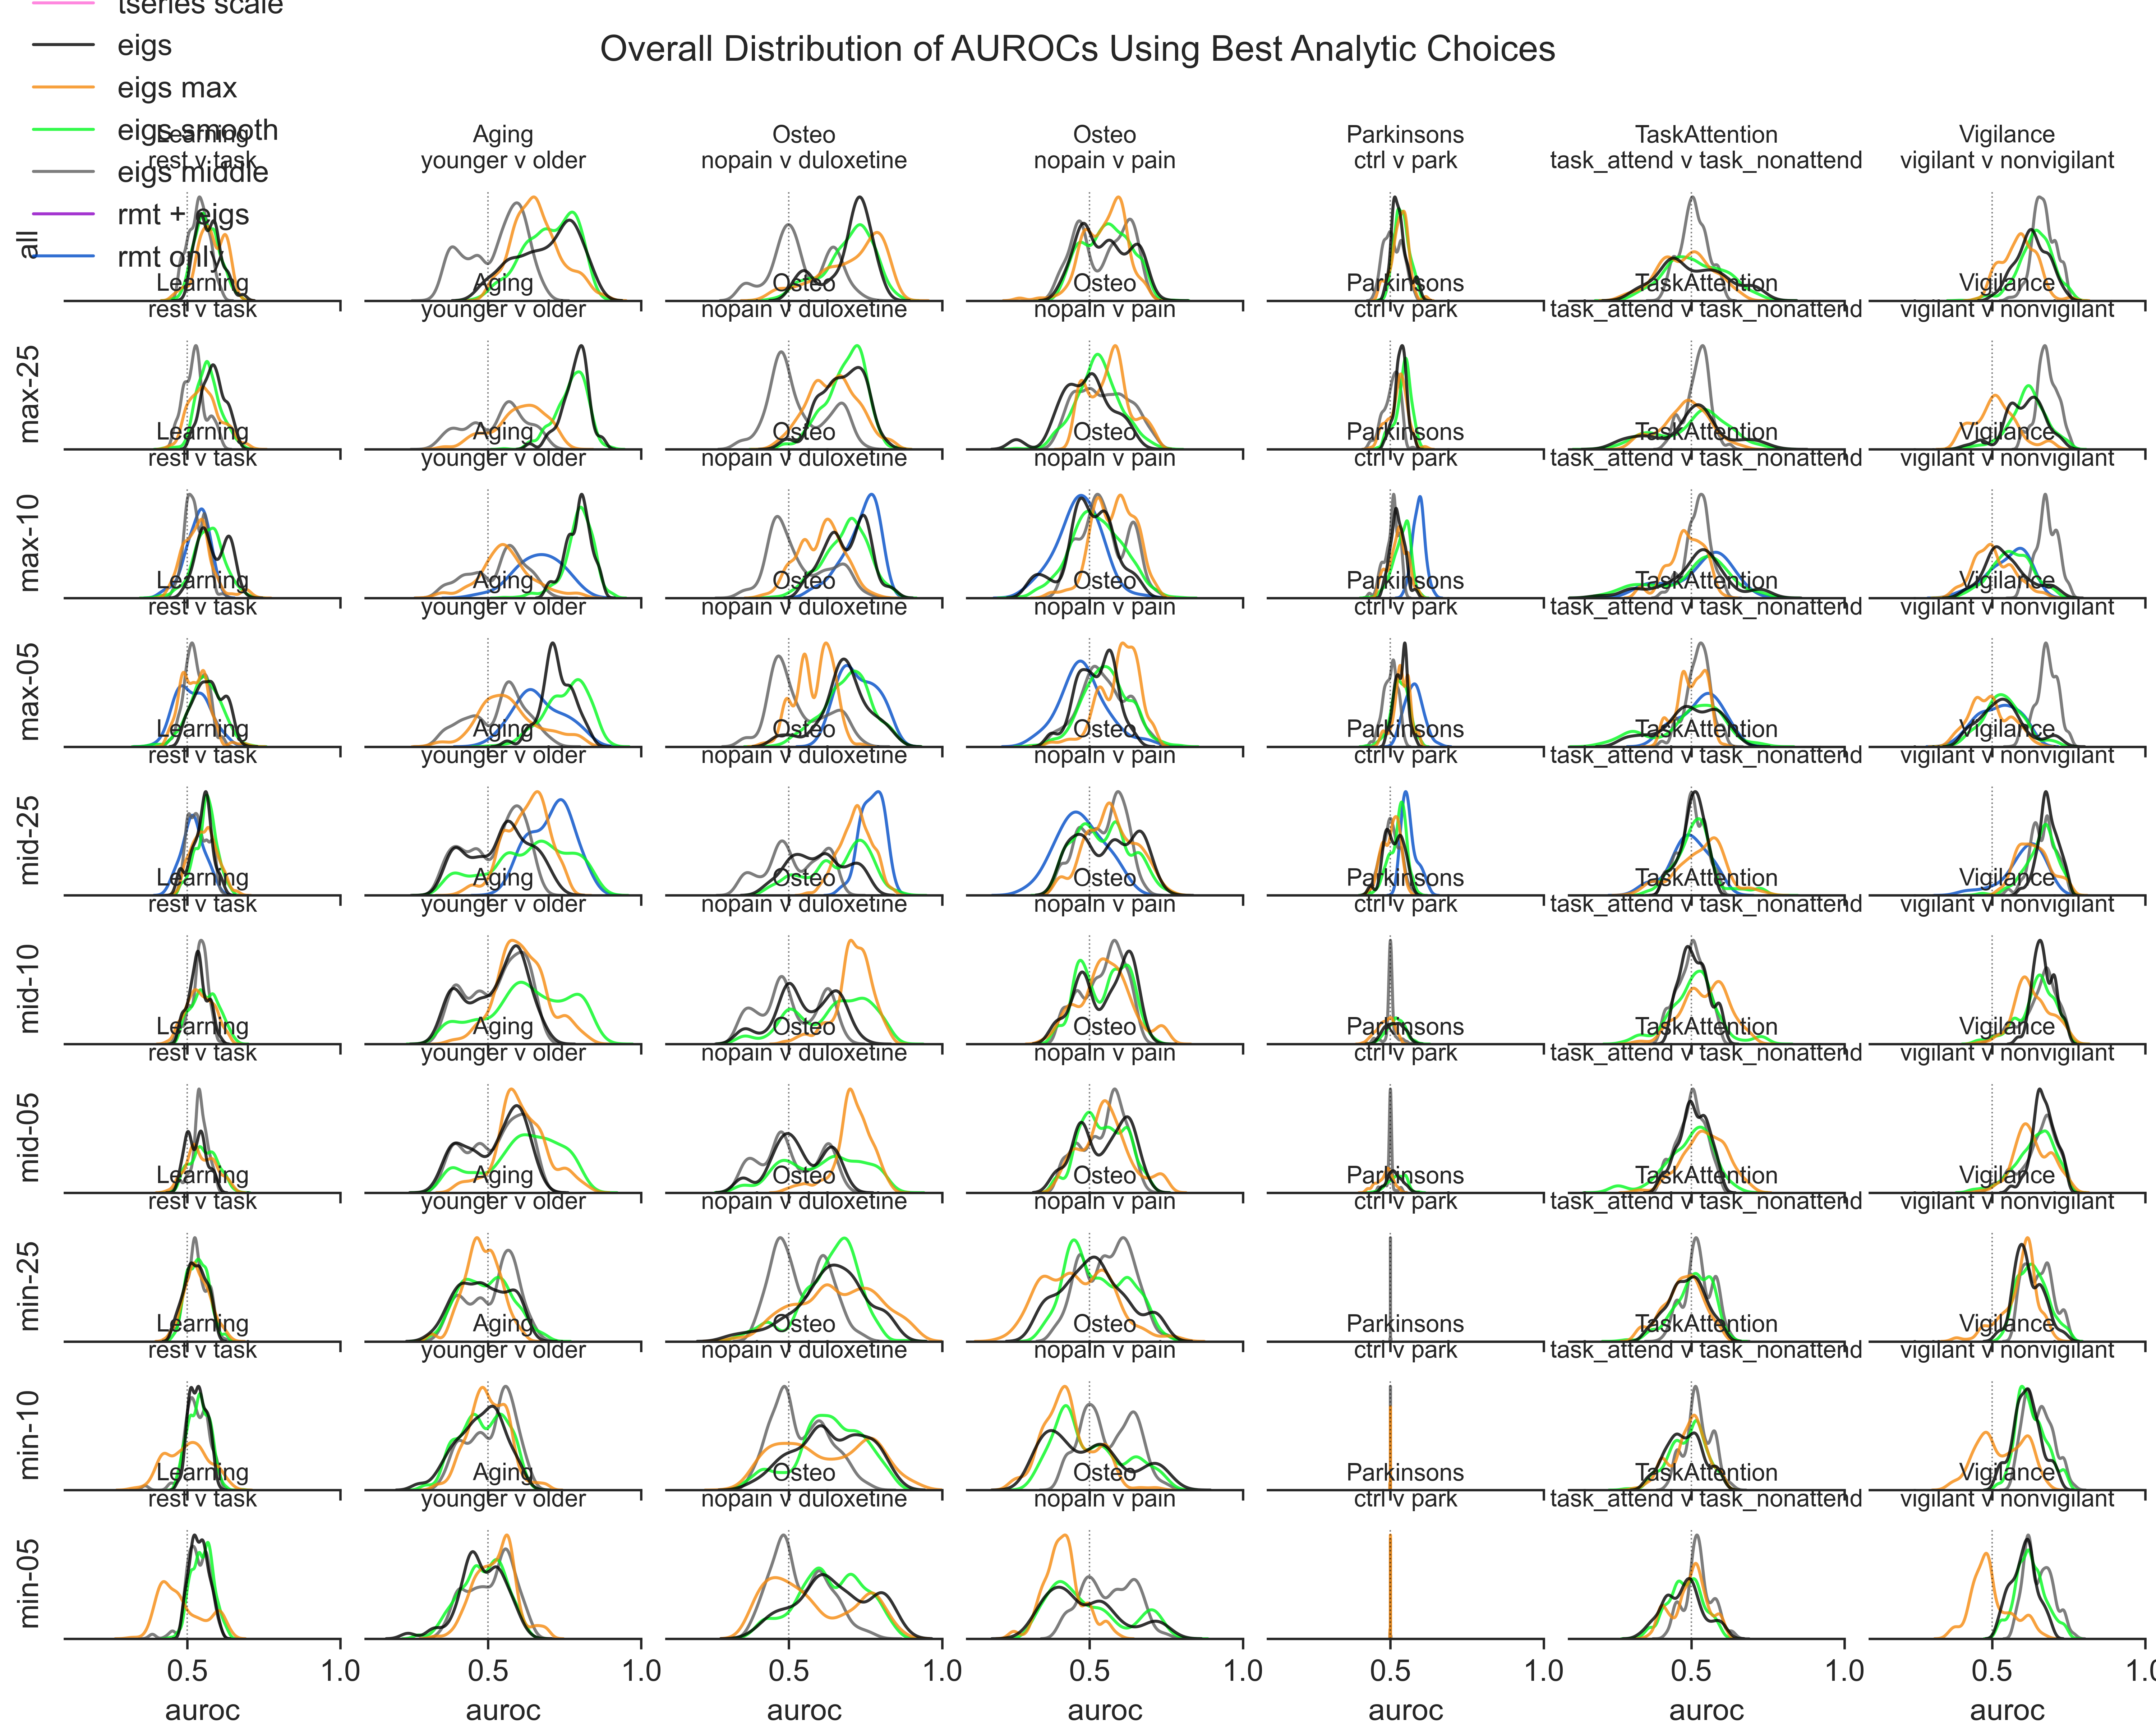
\includegraphics[width=\textwidth,height=0.9\textheight,keepaspectratio]{best_rmt_params_by_subgroup.png}
% \end{center}
% \caption
% { \label{fig:best-params}
% Distributions of mAUROCs when choosing ``best'' analytic choices and features.}
% \end{figure}



%%%%%%%%%%%%%%%%%%%%%%%%%%%%%%%%%%%%%%%%%%%%%%%%%%%%%%%%%%%%%%%%%%%%%%%%%%%%%%%%%%%%%%%%%%%%%%%%%%%
% BEGIN ACC+ FIGURES
%%%%%%%%%%%%%%%%%%%%%%%%%%%%%%%%%%%%%%%%%%%%%%%%%%%%%%%%%%%%%%%%%%%%%%%%%%%%%%%%%%%%%%%%%%%%%%%%%%%

\begin{figure}[H]
\begin{center}
\includegraphics[width=\textwidth,height=0.9\textheight,keepaspectratio]{all_accs_by_fine_feature_groups.png}
\end{center}
\caption
{ \label{fig:feature-group-all-acc} Adjusted accuracy distributions across
fine feature groupings and comparison tasks.}
\end{figure}





\begin{figure}[H]
\begin{center}
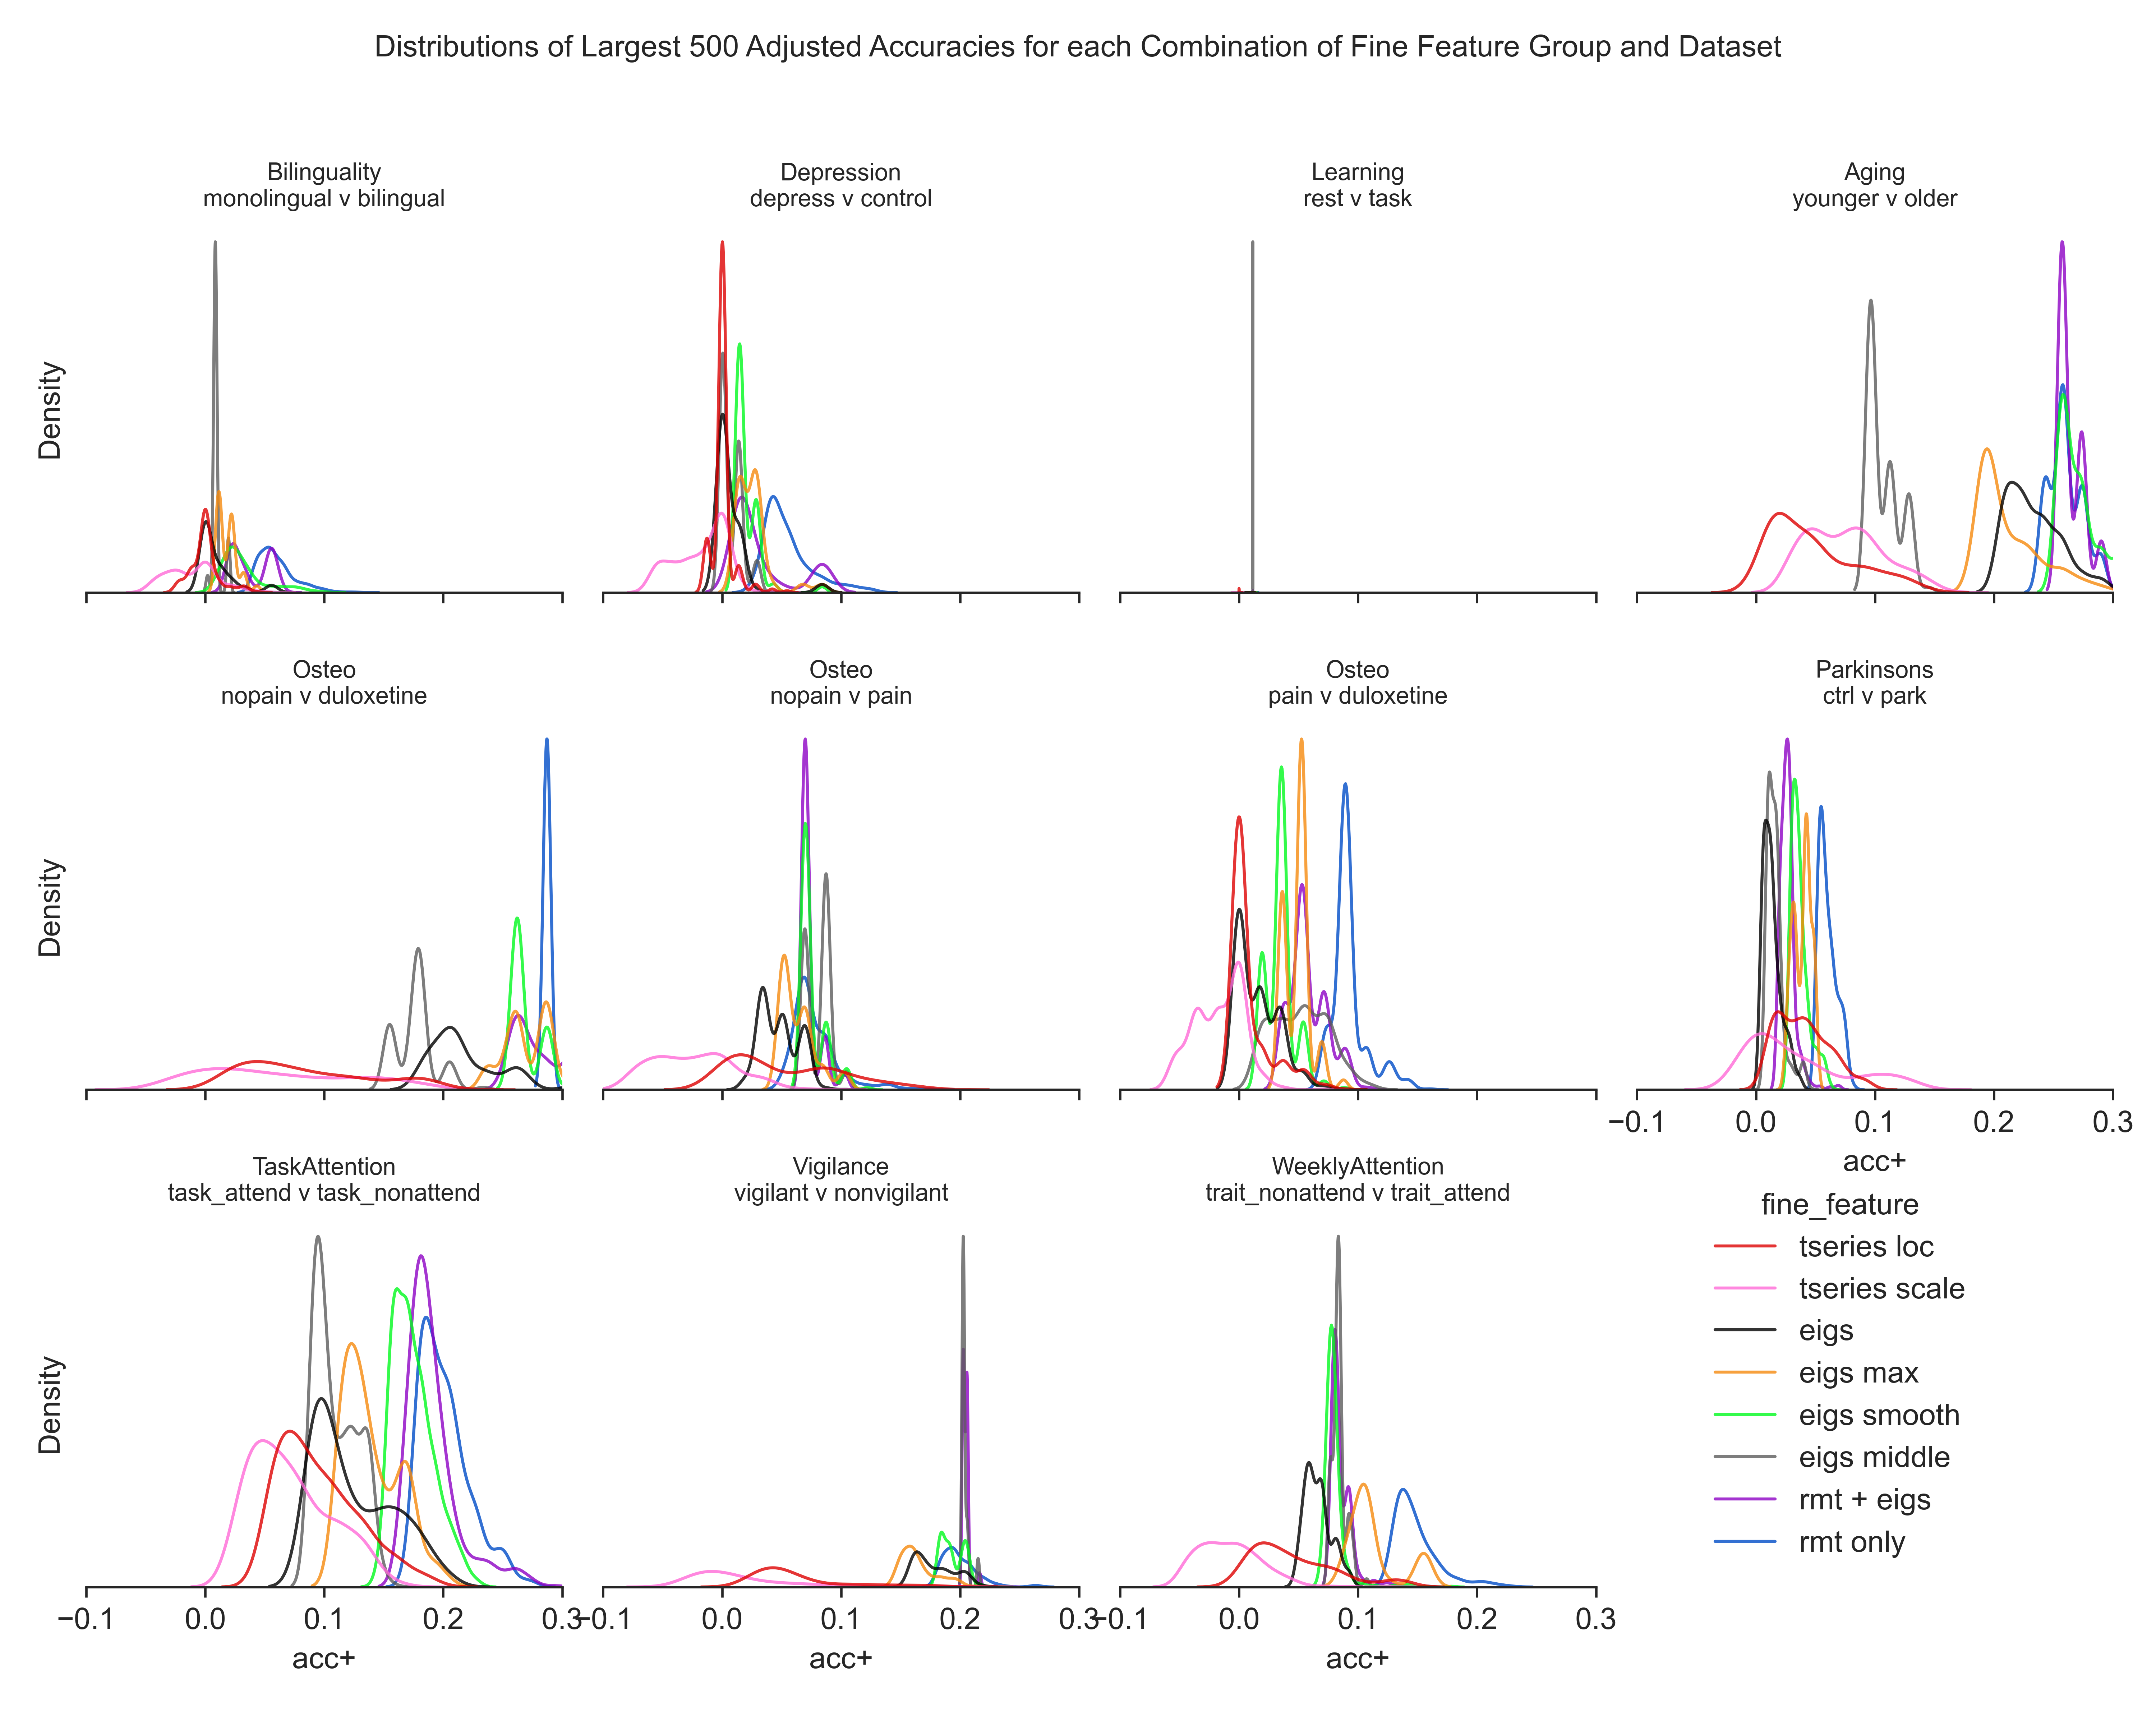
\includegraphics[width=\textwidth,height=0.9\textheight,keepaspectratio]{fine_feature_largest_accs_by_subgroup.png}
\end{center}
\caption
{ \label{fig:fine-largest-acc} Distributions of largest 500 mean adjusted
accuracies across fine feature grouping, by comparison task. Note "rmt only"
and "rmt + eigs" features tend to have the best possible performances across
predictable tasks. }
\end{figure}



\begin{figure}[H]
\begin{center}
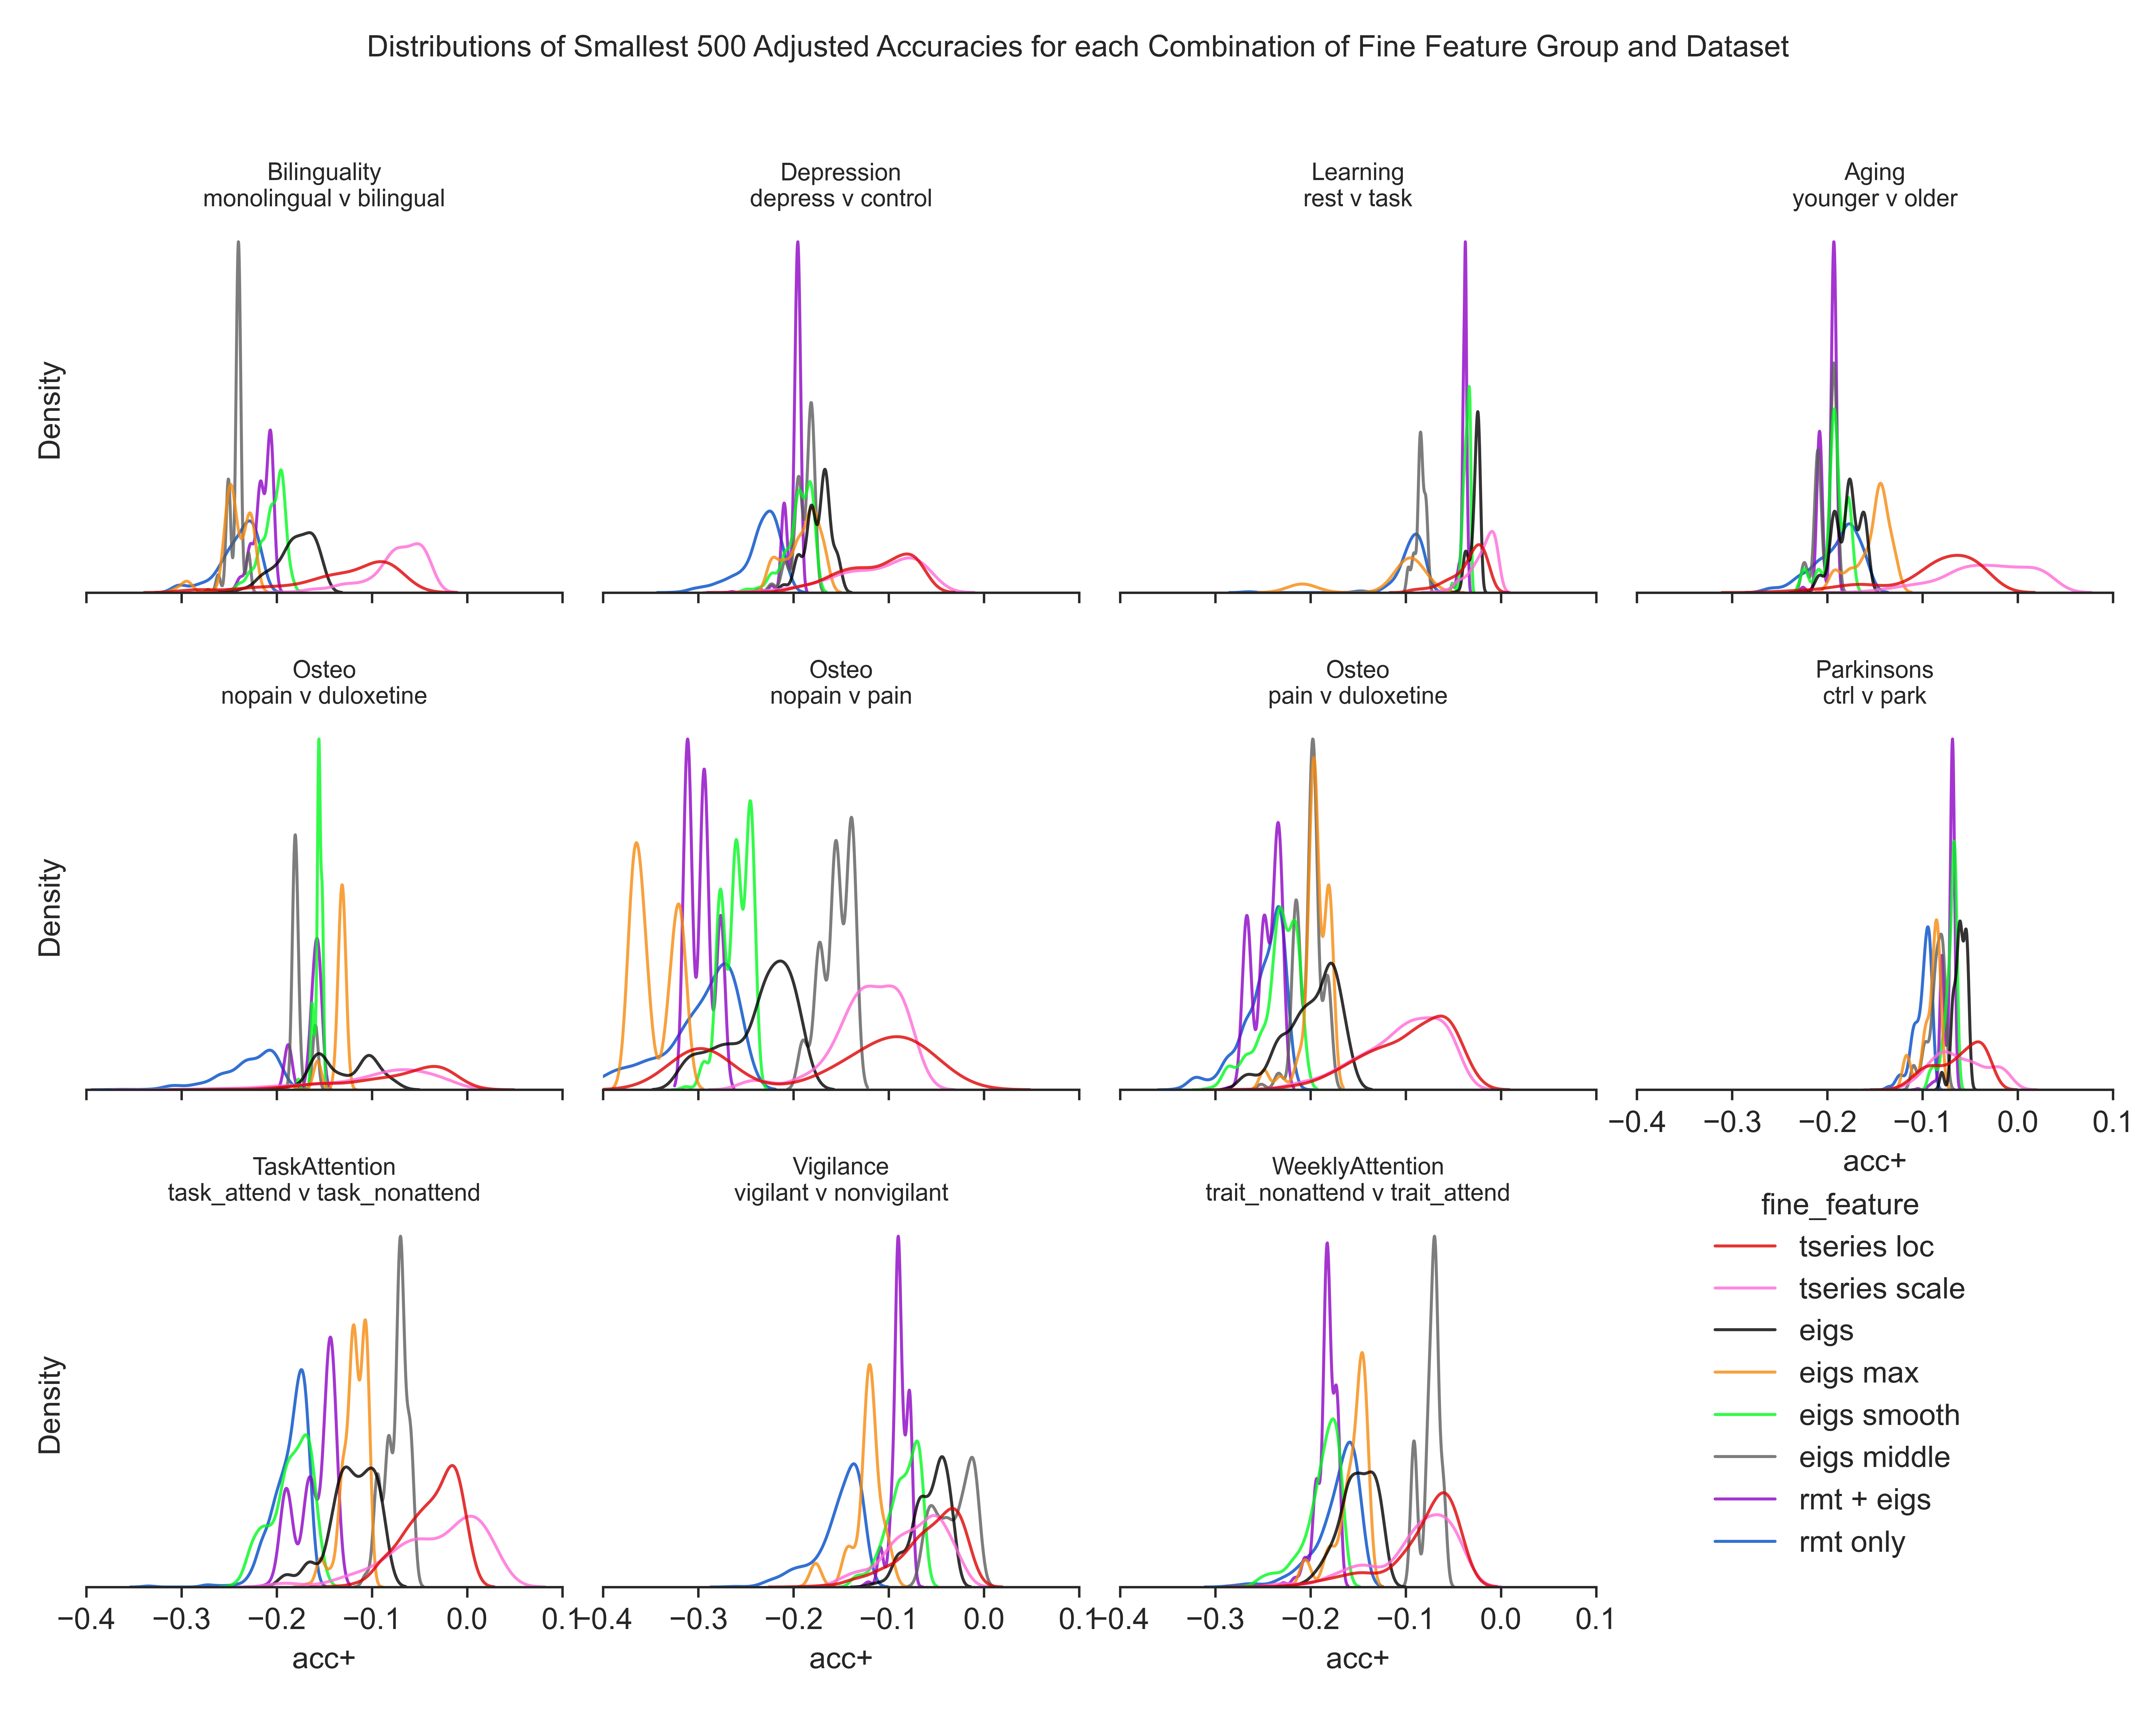
\includegraphics[width=\textwidth,height=0.9\textheight,keepaspectratio]{fine_feature_smallest_accs_by_subgroup.png}
\end{center}
\caption
{ \label{fig:fine-smallest-acc} Distributions of smallest 500 mean adjusted
accuracies across fine feature groupings, by comparison task. Note "rmt only"
and "rmt + eigs" features tend to have the worse possible performances across
predictable tasks.}
\end{figure}


\begin{figure}[H]
\begin{center}
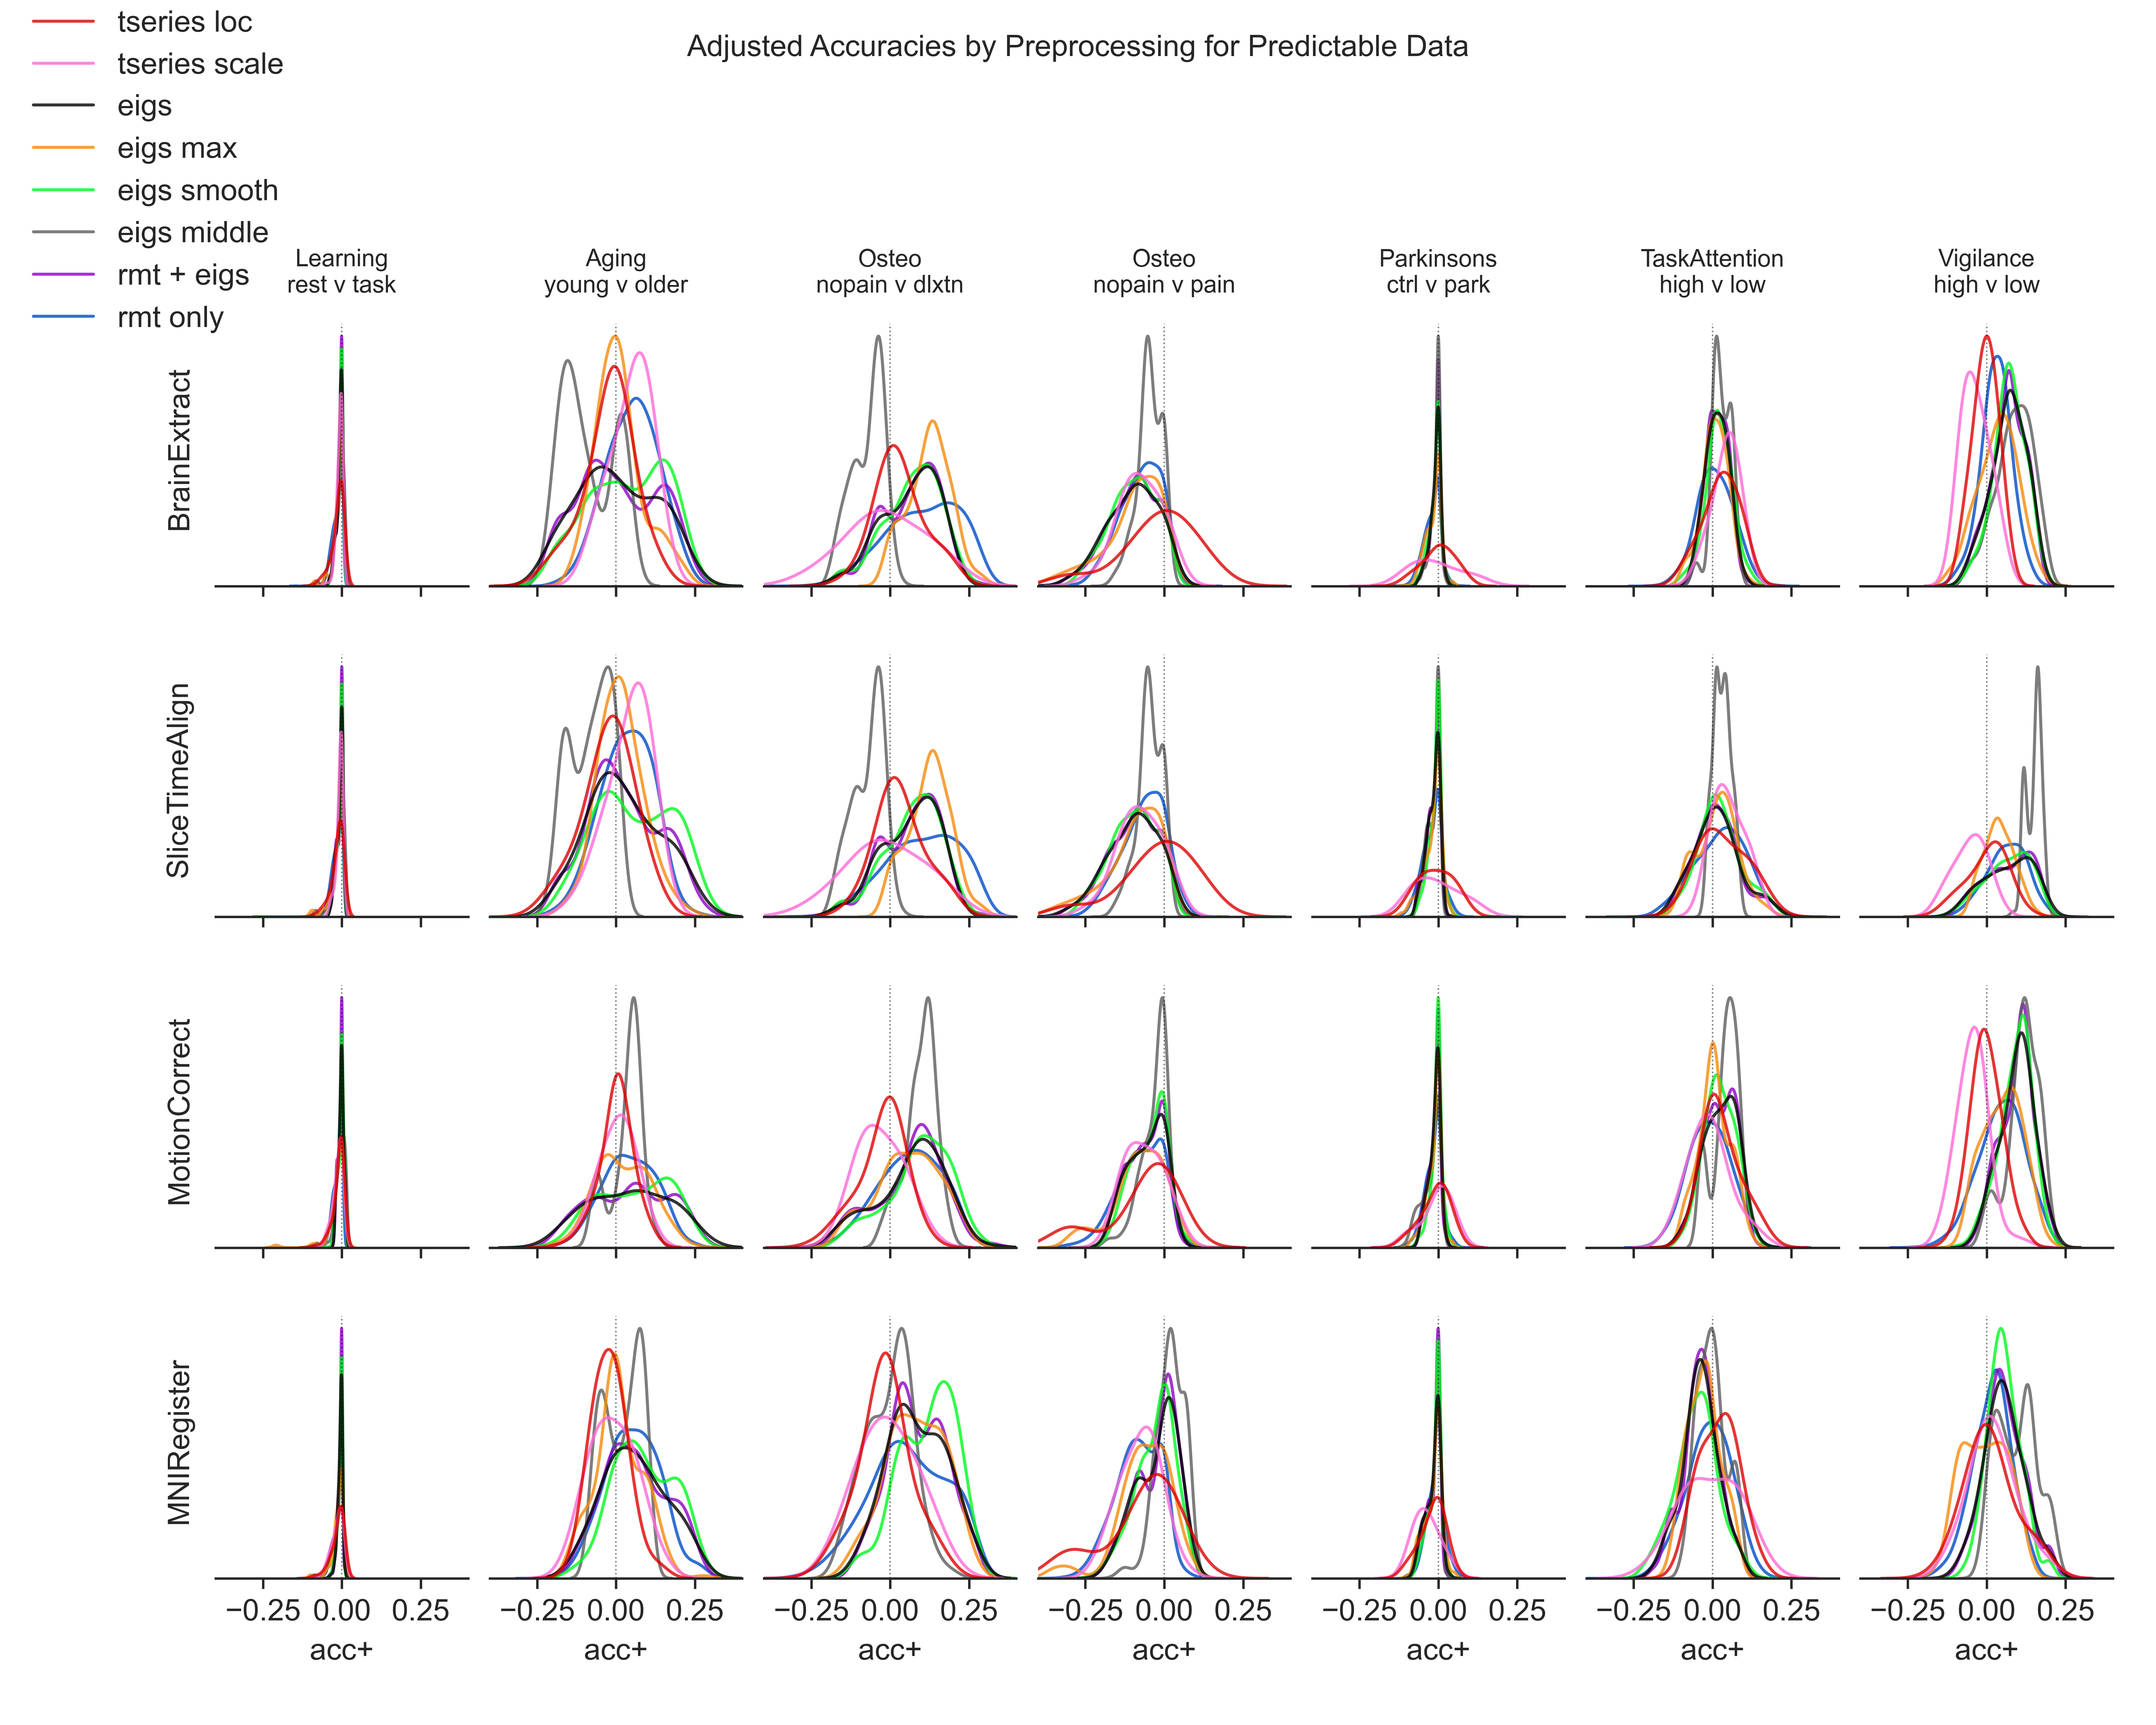
\includegraphics[width=\textwidth,height=0.9\textheight,keepaspectratio]{fine_feature_accs_by_preproc_predictive_subgroup.png}
\end{center}
\caption
{ \label{fig:fine-preproc-acc} Adjusted accuracy distributions across fine
feature groupings and predictable comparison tasks, with effect of
preprocessing.}
\end{figure}


\begin{figure}[H]
\begin{center}
\includegraphics[width=\textwidth,height=0.9\textheight,keepaspectratio]{coarse_feature_group_accs_by_predictive_subgroup_classifier.png}
\end{center}
\caption
{ \label{fig:coarse-classifier-acc} Adjusted accuracy distributions across
coarse feature groupings and predictable comparison tasks, by classifier. Note
the general similarity of each distribution within a particular classification
task (column) and within each feature grouping.}
\end{figure}



\begin{figure}[H]
\begin{center}
\includegraphics[width=\textwidth,height=0.9\textheight,keepaspectratio]{fine_feature_group_accs_by_predictive_subgroup_classifier.png}
\end{center}
\caption
{ \label{fig:fine-classifier-acc} Adjusted accuracy distributions across fine
feature groupings and predictable comparison tasks, by classifier. Note the
general similarity of each distribution within a particular classification task
(column) and within each feature grouping. Note also that, within a
classification task (column), that the rank ordering of features, based on
wither the median, mode, or mean, does not change dramatically or consistently
from classifier to classifier. }
\end{figure}

\begin{figure}[H]
\begin{center}
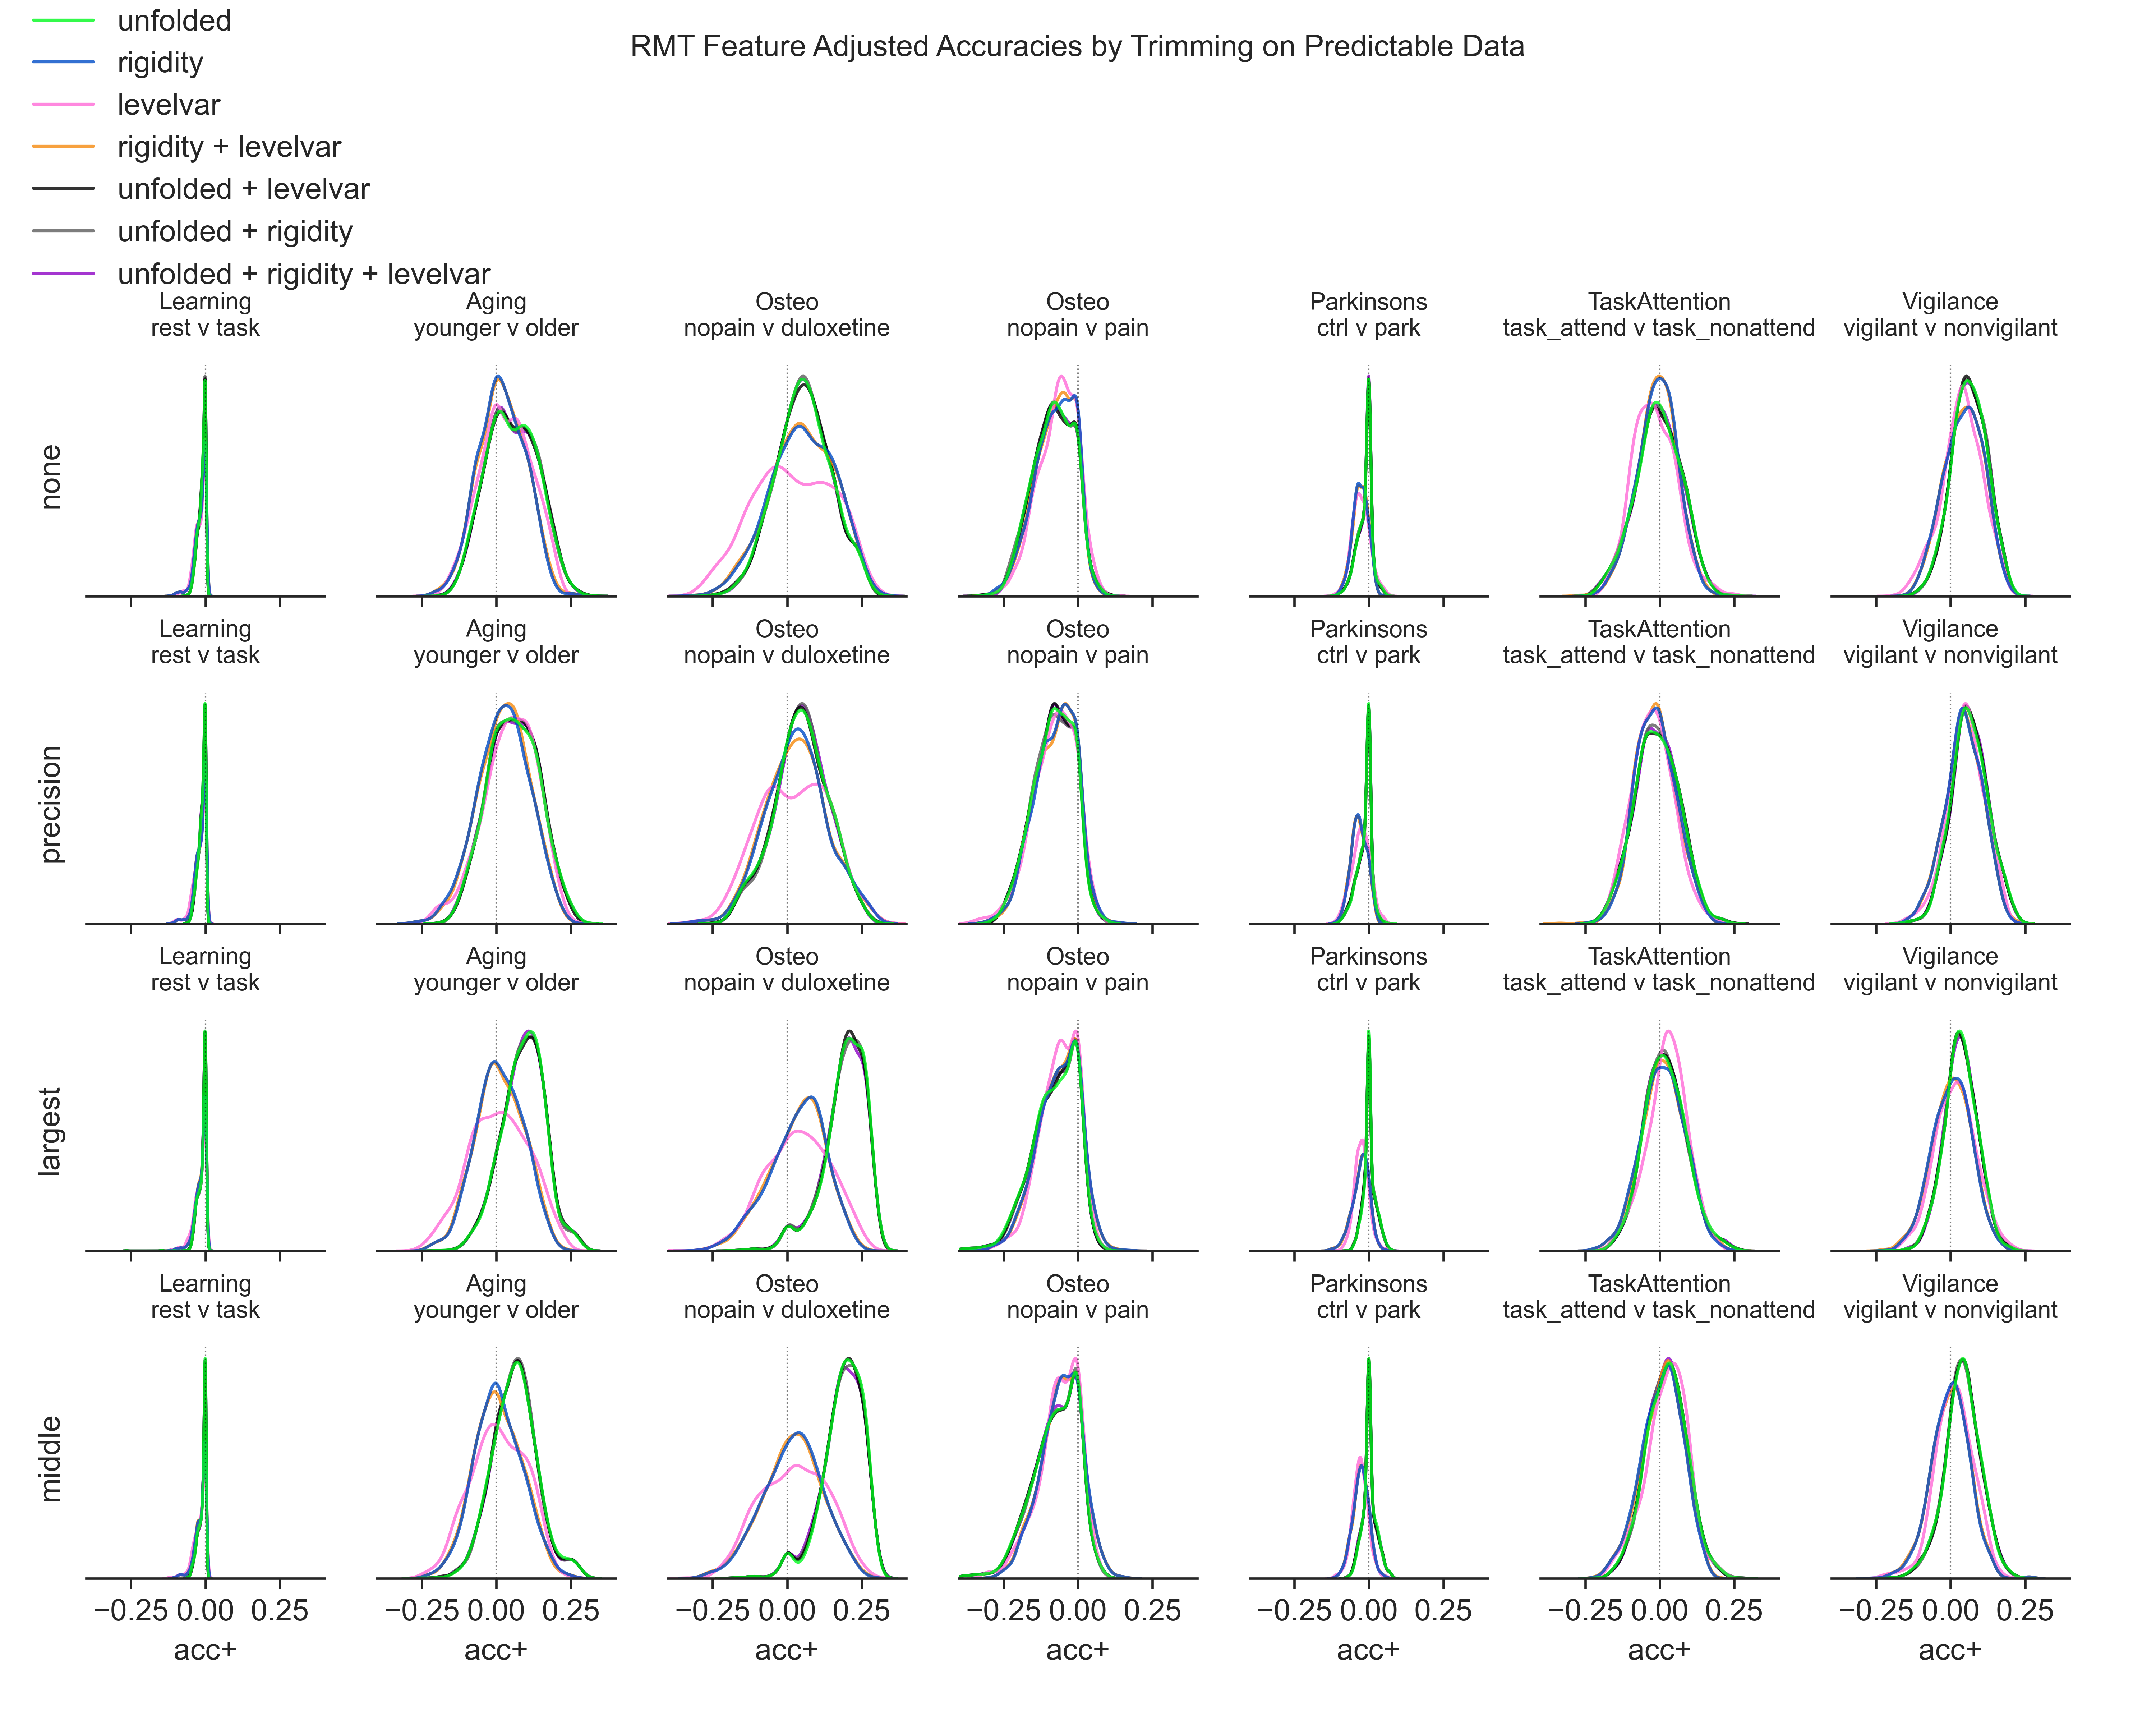
\includegraphics[width=\textwidth,height=0.9\textheight,keepaspectratio]{rmt_feature_accs_by_trim.png}
\end{center}
\caption
{ \label{fig:fine-trim-acc} Distributions of mean adjusted accuracies for
unfolding-dependent RMT features, by trimming. Note the tendency for a
rightward shift in the distributions of the features involving the
unfolded eigenvalues when using largest or middle trimming (most dramatic in
the Osteo nopain v duloxetine condition). The impact of these trimming methods
on the rigidity and level variance features, however, was mixed (compare
Vigilance data to Osteo nopain v duloxetine condition.)}
\end{figure}



\begin{figure}[H]
\begin{center}
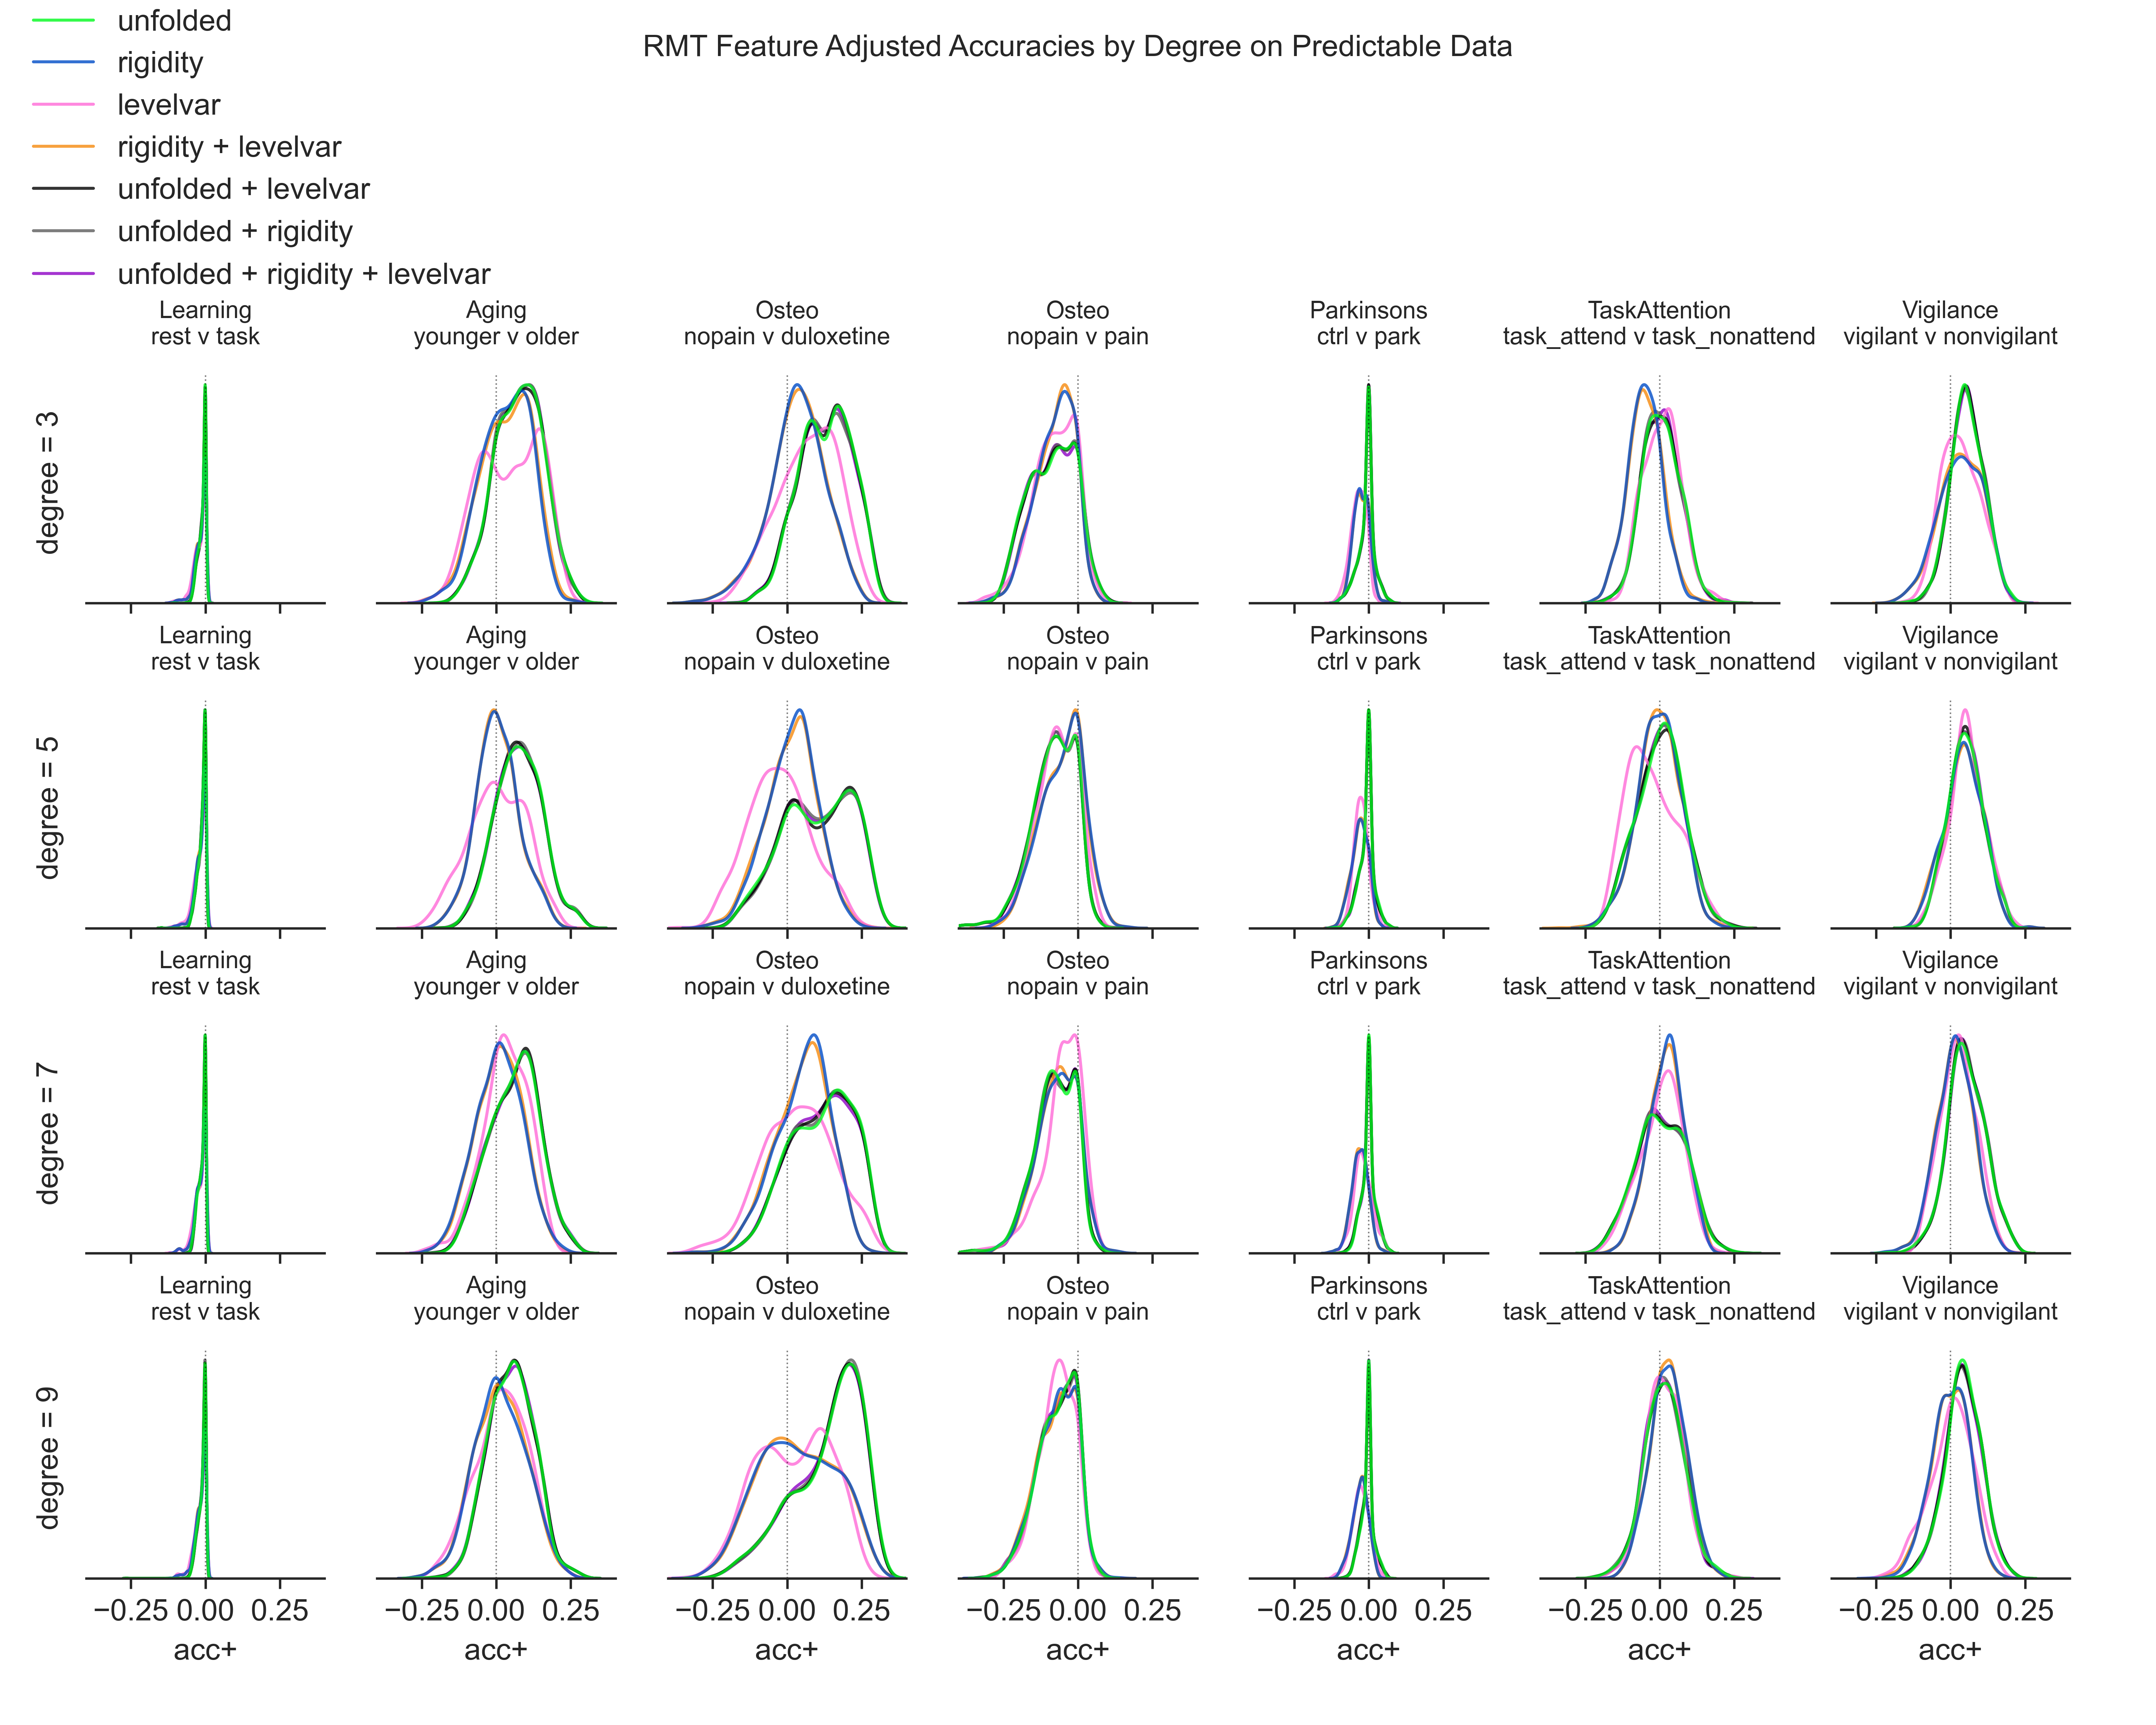
\includegraphics[width=\textwidth,height=0.9\textheight,keepaspectratio]{rmt_feature_accs_by_degree.png}
\end{center}
\caption
{ \label{fig:fine-degree-acc}
Distributions of mean adjusted accuracies for unfolding-dependent RMT features, by degree.}
\end{figure}


\begin{figure}[H]
\begin{center}
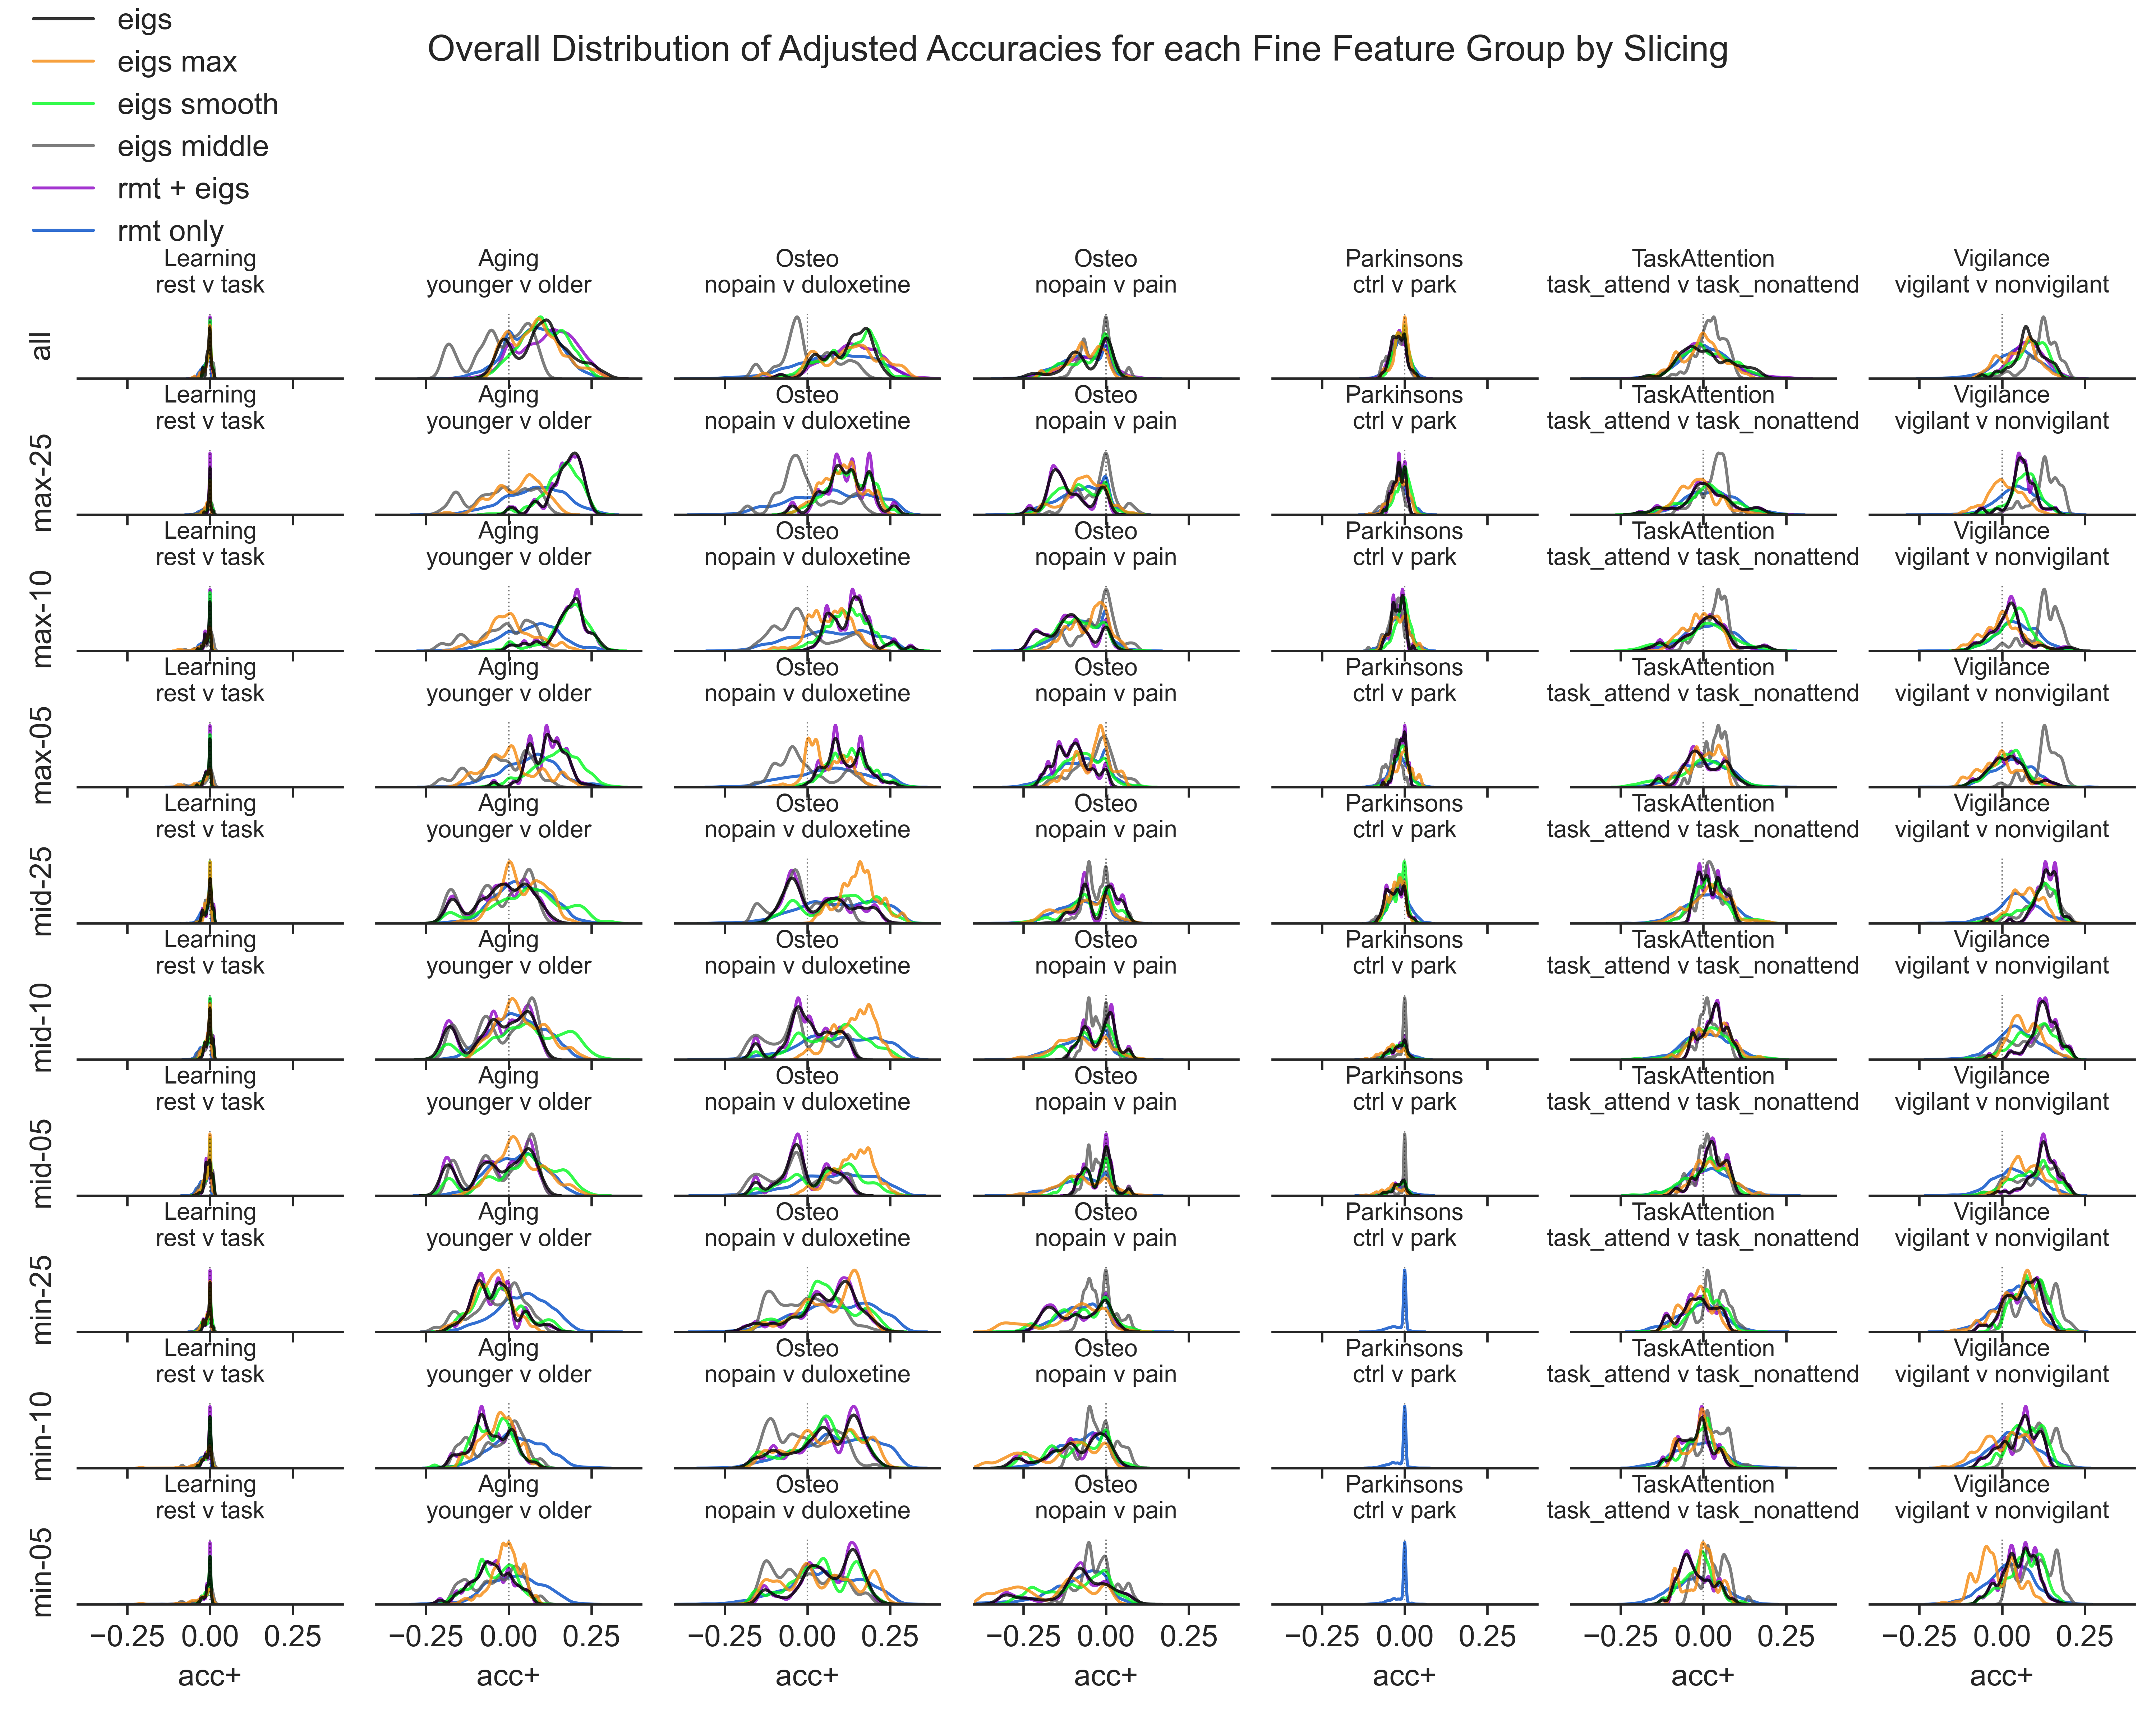
\includegraphics[width=\textwidth,height=0.9\textheight,keepaspectratio]{rmt_eigs_accs_by_subgroup_and_slicing.png}
\end{center}
\caption
{ \label{fig:best-params-slicing-acc} Distributions of mean adjusted accuracies
by slicing. Features involving the full spectrum (raw eigenvalues, smoothed
eigenvalues, and rmt + eigs) sometimes have most positive adjusted accuracy
distributions when using the larger eigenfeature values (first two columns)
or middle values (Osteo nopain v pain condition, Vigilance classification
task).}
\end{figure}




\begin{table}[H]
\caption{Numerical summaries of feature mean accuracy difference from guess
across predictable comparisons, and all combinations of analytic choices,
sorted by 95\% percentile (robust max) value.}
\label{tab:acc-numerical}
\small
\centering

\begin{tabular}{lrrrrrrr}
\hline
Feature &      mean &       min &        5\% &       50\% &       95\% &       max &       std \\
\hline
unfolded                       &  0.021 & -0.437 & -0.123 &  0.000 &  0.196 &  0.312 &  0.091 \\
unfolded + levelvar            &  0.021 & -0.437 & -0.122 &  0.000 &  0.195 &  0.312 &  0.091 \\
unfolded + rigidity            &  0.021 & -0.437 & -0.122 &  0.000 &  0.194 &  0.312 &  0.091 \\
unfolded + rigidity + levelvar &  0.021 & -0.437 & -0.123 &  0.000 &  0.193 &  0.312 &  0.090 \\
eigs + eigs\_smooth             &  0.025 & -0.295 & -0.125 &  0.000 &  0.193 &  0.337 &  0.091 \\
eigs + savgol                  &  0.022 & -0.295 & -0.125 &  0.000 &  0.190 &  0.337 &  0.091 \\
eigs + unfolded                &  0.014 & -0.311 & -0.130 &  0.000 &  0.173 &  0.362 &  0.087 \\
eigs + rigidity + levelvar     &  0.013 & -0.311 & -0.130 &  0.000 &  0.173 &  0.362 &  0.086 \\
eigs + unfolded + levelvar     &  0.013 & -0.311 & -0.130 &  0.000 &  0.173 &  0.362 &  0.087 \\
eigs + unfolded + rigidity     &  0.013 & -0.311 & -0.130 &  0.000 &  0.173 &  0.362 &  0.086 \\
eigs\_savgol                    &  0.016 & -0.313 & -0.126 &  0.000 &  0.172 &  0.321 &  0.085 \\
eigs\_smooth                    &  0.018 & -0.263 & -0.123 &  0.000 &  0.172 &  0.323 &  0.084 \\
eigs + levelvar                &  0.013 & -0.311 & -0.131 &  0.000 &  0.171 &  0.321 &  0.086 \\
eigs                           &  0.013 & -0.311 & -0.130 &  0.000 &  0.168 &  0.312 &  0.086 \\
eigs + rigidity                &  0.013 & -0.311 & -0.131 &  0.000 &  0.162 &  0.312 &  0.085 \\
eigsminmax20                   &  0.007 & -0.348 & -0.123 &  0.000 &  0.159 &  0.309 &  0.083 \\
eigsminmax5                    &  0.002 & -0.367 & -0.120 &  0.000 &  0.159 &  0.284 &  0.084 \\
T-p05                          & -0.004 & -0.298 & -0.193 &  0.000 &  0.155 &  0.205 &  0.091 \\
eigsmiddle40                   &  0.008 & -0.225 & -0.114 &  0.000 &  0.151 &  0.234 &  0.074 \\
eigsmiddle20                   &  0.006 & -0.210 & -0.120 &  0.000 &  0.147 &  0.215 &  0.074 \\
eigsminmax10                   &  0.003 & -0.367 & -0.116 &  0.000 &  0.145 &  0.287 &  0.081 \\
levelvar                       & -0.004 & -0.363 & -0.135 & -0.010 &  0.145 &  0.312 &  0.081 \\
T-rrng                         &  0.002 & -0.249 & -0.140 &  0.000 &  0.144 &  0.184 &  0.079 \\
eigsmiddle10                   &  0.004 & -0.224 & -0.127 &  0.000 &  0.136 &  0.206 &  0.074 \\
rigidity + levelvar            & -0.006 & -0.335 & -0.127 & -0.009 &  0.130 &  0.312 &  0.076 \\
rigidity                       & -0.006 & -0.332 & -0.127 & -0.009 &  0.130 &  0.309 &  0.075 \\
T-mean                         &  0.011 & -0.202 & -0.080 &  0.009 &  0.119 &  0.191 &  0.058 \\
T-med                          & -0.006 & -0.259 & -0.102 & -0.002 &  0.114 &  0.194 &  0.065 \\
T-max                          & -0.003 & -0.192 & -0.106 & -0.002 &  0.112 &  0.180 &  0.066 \\
T-rng                          & -0.004 & -0.173 & -0.104 & -0.002 &  0.110 &  0.169 &  0.063 \\
T-iqr                          & -0.030 & -0.313 & -0.152 & -0.025 &  0.103 &  0.202 &  0.077 \\
T-std                          & -0.025 & -0.202 & -0.126 & -0.026 &  0.094 &  0.147 &  0.065 \\
T-p95                          & -0.011 & -0.228 & -0.115 & -0.002 &  0.079 &  0.180 &  0.061 \\
T-min                          & -0.030 & -0.298 & -0.298 & -0.001 &  0.047 &  0.127 &  0.082 \\
\hline
\end{tabular}
\end{table}



% \bibliography{report}   % bibliography data in report.bib
% \bibliographystyle{spiejour}   % makes bibtex use spiejour.bst

% \end{spacing}
\end{document}